% ---- ETD Document Class and Useful Packages ---- %
\documentclass{ucetd}
\usepackage{subfigure,epsfig,amsfonts}
\usepackage{natbib}
\usepackage{amsmath}
\usepackage{amssymb}
\usepackage{amsthm}

% RMarkdown Stuff %

%% Use these commands to set biographic information for the title page:
\title{Co-policing Surrounding the University of Chicago}
\type{Paper}
\university{The University of Chicago}
\location{Chicago, IL}
\author{Adam Shelton}
\department{Computational Social Science}
\division{Social Sciences}
\degree{Master of Arts}
\date{June 2020}
\advisor{Assistant Professor Yanilda María González}
\advisordept{Social Service Administration}
\preceptor{Joshua Mausolf}

\usepackage{hyperref}
\usepackage{longtable}
\usepackage{booktabs}
% Options for packages loaded elsewhere
\PassOptionsToPackage{unicode=true}{hyperref}
\PassOptionsToPackage{hyphens}{url}
%
%\documentclass[]{article}
\usepackage{lmodern}
\usepackage{amssymb,amsmath}
\usepackage{ifxetex,ifluatex}
\ifnum 0\ifxetex 1\fi\ifluatex 1\fi=0 % if pdftex
  \usepackage[T1]{fontenc}
  \usepackage[utf8]{inputenc}
  \usepackage{textcomp} % provides euro and other symbols
\else % if luatex or xelatex
  \usepackage{unicode-math}
  \defaultfontfeatures{Scale=MatchLowercase}
  \defaultfontfeatures[\rmfamily]{Ligatures=TeX,Scale=1}
\fi
% Use upquote if available, for straight quotes in verbatim environments
\IfFileExists{upquote.sty}{\usepackage{upquote}}{}
\IfFileExists{microtype.sty}{% use microtype if available
  \usepackage[]{microtype}
  \UseMicrotypeSet[protrusion]{basicmath} % disable protrusion for tt fonts
}{}
\makeatletter
\@ifundefined{KOMAClassName}{% if non-KOMA class
  \IfFileExists{parskip.sty}{%
    \usepackage{parskip}
  }{% else
    \setlength{\parindent}{0pt}
    \setlength{\parskip}{6pt plus 2pt minus 1pt}}
}{% if KOMA class
  \KOMAoptions{parskip=half}}
\makeatother
\usepackage{xcolor}
\IfFileExists{xurl.sty}{\usepackage{xurl}}{} % add URL line breaks if available
\IfFileExists{bookmark.sty}{\usepackage{bookmark}}{\usepackage{hyperref}}
\hypersetup{
  pdftitle={Co-policing Surrounding the University of Chicago},
  pdfauthor={Adam Shelton},
  hidelinks,
}
\urlstyle{same} % disable monospaced font for URLs
\usepackage[margin=1in]{geometry}
\usepackage{graphicx,grffile}
\makeatletter
\def\maxwidth{\ifdim\Gin@nat@width>\linewidth\linewidth\else\Gin@nat@width\fi}
\def\maxheight{\ifdim\Gin@nat@height>\textheight\textheight\else\Gin@nat@height\fi}
\makeatother

\providecommand{\tightlist}{%
  \setlength{\itemsep}{0pt}\setlength{\parskip}{0pt}}




%% Use these commands to set a dedication and epigraph text

\usepackage{booktabs}
\usepackage{longtable}
\usepackage{array}
\usepackage{multirow}
\usepackage{wrapfig}
\usepackage{float}
\usepackage{colortbl}
\usepackage{pdflscape}
\usepackage{tabu}
\usepackage{threeparttable}
\usepackage{threeparttablex}
\usepackage[normalem]{ulem}
\usepackage{makecell}
\usepackage{xcolor}


% Remove Chapter N Headings and Adjust spacing
\usepackage[compact]{titlesec}

\titleformat{\chapter}[display]
  {\normalfont\bfseries\center}{}{0pt}{\Large\vspace{0pt}}

\titlespacing*{\chapter}{0pt}{-50pt}{0pt}

% Place all figures at end
\usepackage[nolists,heads]{endfloat}

\renewcommand{\efloatseparator}{\mbox{}}

\let\normallongtable=\longtable
\renewcommand{\longtable}{\clearpage\normallongtable}

\DeclareDelayedFloatFlavour*{longtable}{table}

% Maintain figures aspect ratio
\setkeys{Gin}{width=0.8\textwidth,height=0.8\textheight,keepaspectratio}

% Allow box characters for skimr
\usepackage{pmboxdraw}

\begin{document}
%% Basic setup commands
% If you don't want a title page comment out the next line and uncomment the line after it:
\maketitle
%\omittitle

% These lines can be commented out to disable the copyright/dedication/epigraph pages
\makecopyright
\abstract{This paper explores the differences between the Chicago Police
Department and private campus police operated by the University of
Chicago. Both departments share a jurisdiction in the community
surrounding the University operating under equivalent authority to
police the region. This project aims to describe the distinctions
between these two departments by understanding how their reactions to
reported crimes differ. As colleges and universities across the country
expand their police departments, it is increasingly important to
understand not only how these departments operate, but how they affect
the surrounding community members and municipal policing efforts. We
find the University of Chicago Police department supplements municipal
policing by primarily focusing on petty crimes and non-criminal
incidents that are more likely to affect university students and
faculty. However, while the UCPD does collaborate extensively with CPD
on more violent crimes, it is again for crimes that impact stakeholders
at the university more, such as robberies and assaults. This has serious
implications for surrounding neighborhoods, which are predominantly
communities of color, who are not being represented by the UCPD in
policing practices and have no direct power to hold the University
accountable for the actions of its private police force.}


%% Make the various tables of contents
\tableofcontents
\listoffigures
\listoftables

%\acknowledgments
% Enter Acknowledgements here

% Enter Abstract here

\mainmatter
\hypertarget{introduction}{%
\chapter{Introduction}\label{introduction}}

The United States has a complicated history of policing entangled with
racial injustices. Police patrols in the United States can trace their
roots to slave patrols during the formative years of the country (Capers
2009; Sklansky 1999). These white vigilante groups used fear and
intimidation tactics to exert control over slaves and those thought to
be helping them (Sklansky 1999). During the period of Jim Crow laws,
blacks still endured police intimidation and brutality, justified
through laws designed to relegate black Americans to the bottom of the
social order (Wynes 1967; Ross 1983). However, these punitive measures
were not applied equally, with police rarely charging those who
participated in lynch mobs against people of color (Ross 1983). These
inequities still echo through policing today, with minorities and
inhabitants of low-income areas experiencing documented over-policing,
mass incarceration, and increased police violence (Tuch and Weitzer
1997; Weitzer 2000; Alpert et al. 2006).

Across the country public and private policing efforts have grown to
counter criminal activity (Strom et al. 2010; Sklansky 1999). Many
businesses hire or contract security guards to protect their
establishments, goods, and customers (Strom et al. 2010). These
personnel typically operate within extremely narrow bounds, with limited
jurisdiction and the ability to exert force (Sklansky 1999). These
security guards are typically intended to act as a deterrent and
trustworthy witness of criminal activity, rather than intervening force
(Sklansky 1999).

However, organizations or individuals can hire private police forces
that are able to operate with much wider latitude (Sklansky 1999). Many
states allow for armed private police with fully equipped patrol cars
(Strom et al. 2010; Sklansky 1999). Increasingly, universities are
operating their own police departments with this kind of far-reaching
authority (Strom et al. 2010; Reaves 2015). Yet, while public
universities must maintain some amount of transparency, and are
susceptible to FOIA requests, private universities are under no
obligation to provide information if requested (Newman 2016). Therefore,
private universities have the ability to operate, in many cases quite
large, police forces with little to no accountability and oversight.
Under Illinois state law, the police departments of private
universities, are only beholden to the university's Board of Trustees,
not the communities on or off campus that they police (110 ILCS 1020,
n.d.).

Considering the long-running entanglement of racism and violence with
policing, the combination of far-reaching authority, lack of
accountability and oversight, abundance of resources, and interaction
with vulnerable populations typically found at private universities is
alarming. There are few better places to study possible inequities as a
result of private university policing than at the University of Chicago,
which has an extensive history of supporting gentrification efforts to
push out people of color in Hyde Park (Sherman 2019; Larson 2012). The
campus in Hyde Park is surrounded by lower income neighborhoods,
predominantly composed of people of color, which are policed by the
University of Chicago Police Department (UCPD) (Sherman 2019). The UCPD
has been accused of racially biased policing practices, which have been
exhibited in data on stops released by the university (Newman 2016). As
the UCPD and Chicago Police Department (CPD) both share jurisdiction,
this offers us a unique opportunity to observe the interactions of
public and private police forces and their respective inequities.

\hypertarget{literature-review}{%
\chapter{Literature Review}\label{literature-review}}

\hypertarget{inequity-in-policing}{%
\section{Inequity in Policing}\label{inequity-in-policing}}

Since the 1970's, mass incarceration produced by an increase in punitive
policing, such as the War on Drugs, have been used to perpetuate racial
injustices, with ``African Americans are incarcerated at nearly six
times the rate of whites, and Hispanics are incarcerated at almost twice
the rate of whites'' (Fortner 2015). America still lives in segregated
communities, leading to separated communities of color exhibiting higher
crime rates, not due to residents but the lack of jobs, education, and
other opportunities (Capers 2009). The absence of social capital
``\ldots that can increase the likelihood of upward mobility is likely
to be self-perpetuating\ldots{}'' (Capers 2009). This leads to higher
unemployment and lower property values in minority neighborhoods, which
coupled with decreased trust and perceived legitimacy of police
officers, can exacerbate issues of crime and policing in these
communities (Capers 2009).

This creates serious consequences for all people, but especially affects
those in society that are already disadvantaged. There is a long history
of public policing being racialized or otherwise not applied equally
across the population (Alpert et al. 2006; Tuch and Weitzer 1997).
Communities of color have been consistently more likely to be subjected
to excessive force, exacerbating inequality through social
ramifications, like distrust for police and authority (Tuch and Weitzer
1997). Residents in black neighborhoods are also more likely to say that
``police stop people in the neighborhood without good reason, verbally
abuse neighborhood residents, and and use excessive force against
neighborhood residents'' (Weitzer 2000). These problems exist in public
police departments across the country, but often goes unaddressed, as
white people are less likely to think racism in policing exists (Tuch
and Weitzer 1997; Weitzer 2000). Yet, in many areas, white officers make
up a greater proportion of the police force (Tuch and Weitzer 1997) and
are more likely to give out tickets (Alpert et al. 2006). Due to high
levels of racial segregation, white police officers are likely to come
from predominately white neighborhoods, while predominately interacting
with people of color only on patrol, which can reinforce stereotypes and
racialized policing (Capers 2009).

Gentrification, while reducing the intensity of policing in the
immediate area, can increase policing activity outside of the
gentrifying area (Laniyonu 2018). However, despite a decrease in
policing, it appears crime increases in gentrifying areas (Laniyonu
2018). While Broken Windows policing, which focused on reducing physical
disorder in an attempt to reduce crime, was very popular during the
1980's and 1990's, there is contradictory evidence about its
effectiveness (Laniyonu 2018). Likely due to the stereotypical
associations of people of color and poor with crime, there is strong
evidence that the proportion of black Americans in an area is correlated
with the distribution of police officers (Laniyonu 2018; Capers 2009)

Typically, the decision-making by police officers leading up to a stop
is driven by a person appearing ``different'' or ``out of place''
(Alpert et al. 2006). As a result, minorities are frequently stopped in
white neighborhoods, despite data showing that police suspicions about
criminality in most stop and frisks are wrong (Capers 2009). Policing
guided by these philosophies invites bias into the policing process,
resulting in the targeting of males and minorities (Alpert et al. 2006).
Policing that does not adequately address the concerns of the community,
expectedly can have as detrimental effects on the community as crime can
(Daniel and Moynihan 1970). While crime drives down patronage of
businesses, churches, and community organizations, that communities of
color revolve around, ineffective policing only increases feelings of
danger in the community (Daniel and Moynihan 1970). Policies that
emphasize transparency and accountability in policing to the community
are not only comforting to residents but result in more effective
enforcement of laws.

\hypertarget{private-policing}{%
\section{Private Policing}\label{private-policing}}

Despite racial and socioeconomic tensions in policing, and a historical
distrust of private police, there is a large and growing industry
surrounding private policing. In 2015, companies spent approximately
\$30 billion on private security (Pappas 2012). The United States
Department of Labor estimated that in 2018 1.15 million people in the
United States were employed as Security Guards or Gaming Surveillance
Officers (US Department of Labor 2018). Guarding represents
approximately half of all private security services, with 35 percent of
services utilizing armed guards (Strom et al. 2010). Retail,
restaurants, and food service was the industry sector with the highest
percentage of security officers per employees in 2009 at about 17
percent (Strom et al. 2010). Colleges and universities were ranked tenth
with a four percent ratio of security officers to employees (Strom et
al. 2010). The State of Illinois requires that any private detective,
private security contractor, private alarm contractor, fingerprint
vendor, or locksmith be licensed by the state (225 ILCS 447 2004).
However, it is likely for these measurements to be \emph{underestimates}
of the size of private policing (Sklansky 2011). Quantitatively
measuring the scope of private police is incredibly difficult, due to
the secrecy and ambiguity surrounding the number of employees performing
security work (Sparrow 2014; Sklansky 2011).

With private police these issues with accountability and
representativeness become even more difficult to address, especially as
they have become a more integral part of society. In the United States,
there has been considerable growth in private policing in the last half
century, sparking questions about the motivations of these private
forces (Shearing 1992). It is now common for public and private police
departments to collaborate within their jurisdictions (Shearing 1992;
Sparrow 2014), effectively creating a ``network of public police and
private security that is often overlapping, complimentary {[}sic{]} and
mutually supportive'' (Bouthillier et al. 2006). As governments have
sought to cut costs, and private organizations have seen it more cost
effective to hire their own workforce for protection, there has been a
shift in social control out of the public sphere (Shearing 1992; Joh
2006).

Americans quickly became disillusioned of private policing in the early
years of the mining and railroad industries. Private police forces used
by the companies in these industries lead to a protection of assets over
employees and went against the public interest (Spitzer and Scull 2011;
Joh 2006). This resulted in a long period where the state held a
``monopoly'' on policing. However, starting in the 1960's private
policing began to expand, partly in response to a RAND report that
re-framed private policing as ``an `industry' providing a `service'\,''
(Shearing 1992; Joh 2006).

Supporters of this expansion of private police forces claimed that
public police had not been provided enough resources to adequately
patrol their jurisdictions, creating this ``vacuum'' which private
police were filling. This was framed as a win for everyone, as private
police were now performing a role which taxpayers needed but also did
not have to fund, and regulations would limit their power (Shearing
1992; Joh 2006). Critics were concerned that now companies could give
employees ``state authority'', and that this cooperation between
governments and corporations would only protect the interests of the
elite (Shearing 1992).

In recent history, private policing within corporations has shifted to
focus on investigative labor (Spitzer and Scull 2011). This shift
represents a growing emphasis on obtaining ``restitution'' versus
``revenge'' (Spitzer and Scull 2011). Thorough investigations allow for
a better likelihood of restitution through legal means, while minimizing
the risk of valuable information becoming public (Spitzer and Scull
2011). However, any company's goal is to maximize profits, which means
occasionally relying on public police, as that incurs no costs to the
company (Spitzer and Scull 2011).

Privatized police officers are particularly problematic when it comes to
accountability, as there is a much lower legal standard for how private
forces should operate. Private police forces are now under much less
government scrutiny, as public police departments rely on the
partnership they have with private forces (Joh 2006). Citizens also have
fewer legal protections from private police, who are not under any
constitutional obligation to follow due process regulations (Sklansky
1999). This means that private police forces are not obligated to
provide Miranda warnings before interrogation, and evidence discovered
by a search is almost always admissible, although the officer could be
charged with assault, trespassing, or false imprisonment (Sklansky
1999).

Yet, despite this lack of regulation, private police officers often have
the same or similar powers of public police, over that of which other
citizens have (Sklansky 1999). Additionally, private police forces
formed by companies are oftentimes allowed to sit in on regional or
federal task forces, giving companies access to sensitive information
they did not have before (Joh 2006).

This creates far-reaching implications, especially in the case of
university police forces, where private police patrol large areas
outside of the campus. When these officers have the power to police
citizens other than students, there is little to no oversight on whether
this power is being exercised fairly and justly, which is antithetical
to the strict limitations imposed on police in the Constitution. There
will always be instances where the interests of private police are
against that of the public's (Sparrow 2014). It is important that
citizens understand when these private forces are acting against the
public's interests, not only to help protect themselves, but to also
spread awareness for this alarming status quo, motivating law makers to
more heavily regulate private police forces.

\hypertarget{campus-policing}{%
\section{Campus Policing}\label{campus-policing}}

Private and public policing has also expanded on college campuses, with
approximately two-thirds of four-year colleges or universities with more
than 2,500 students employ sworn police officers, with 92 percent of
public institutions and 38 percent of private institutions doing so
(Reaves 2015). About three quarters of campus officers overall are armed
and about eight in ten campus officers could arrest and patrol beyond
campus boundaries (Reaves 2015). A larger proportion of police
departments at public institutions met regularly with advocacy groups
than private institutions (Reaves 2015). The increase in law enforcement
personnel has outpaced student enrollment (Reaves 2015). Campuses with
sworn officers, on average employed 2.4 full-time sworn officers per
1000 students, with private institutions having higher ratios than
public institutions (Reaves 2015).

Under the Jeanne Clery Disclosure of Campus Security Policy and Campus
Crime Statistics Act of 1990, institutions of higher education that
participate in federal financial aid programs must keep and disclose
information about crime on and around campus (Reaves 2015; Bauman 2014).
On average, overall crime rates are higher at private institutions, both
both public and private institutions reported handling about 40 violent
crimes per 100,000 students during the 2011-2012 school year (Reaves
2015). Usually, ``sworn officers must undergo a considerably more
rigorous screening process prior to hiring than their non-sworn
counterparts'', but a majority of departments require a college degree
for both types of officer (Reaves 2015). While the proportion of
minority officers and female officers increased from the previous survey
in 2004, the majority of sworn officers were both white and male during
the 2011-2012 school year (Reaves 2015).

In some ways, campus police can better serve the public's interests than
public police departments. While campus police work to maintain a ``good
image'' of the school by enforcing campus rules for students (Jacobsen
2015), they can still benefit the public, sometimes more effectively
than municipal police departments. More small campus agencies were found
to have formed problem-solving partnerships and provided training to
citizens than small city agencies (Bromely 2003). Overall, campus police
feel their job is to keep students safe and make them feel comfortable
(Williams et al. 2016). Police officers employed by universities must
undergo Title IX training as all university employees must, and often
complete more training about sexual harassment than their municipal
counterparts (Smith, Wilkes, and Bouffard 2016). Officers with
specialized training pertaining to sexual crimes typically scored lower
on scales of rape myth acceptance (Smith, Wilkes, and Bouffard 2016).
Perhaps a testament to this focus on safety by campus police, students
generally regard their campus as a ``protected space'' which is safer
than other areas and feel that campus police are responsible for this
safe environment (Williams et al. 2016; Jacobsen 2015).

Yet, while in a 1998 survey of white college students and faculty only
ten percent of respondents felt unsafe on their campus, 36 percent
supported arming campus police officers and an additional 26 percent
were undecided (Hummer, Austin, and Bumphus 1998). Of the 38 percent of
respondents that felt campus police should not be armed, ``50 percent
felt that''campus life" is not that life-threatening and therefore did
not warrant the carrying of firearms by officers" (Hummer, Austin, and
Bumphus 1998). 63 percent of respondents who were undecided felt that
``the use of firearms should be dependent on the severity of the
situation'' (Hummer, Austin, and Bumphus 1998).

Campus police officers also play different roles in the lives of those
within their jurisdiction. Police on campuses often must play the role
of a more parental figure, as most young adults at college are growing
into and adjusting to their first experiences living on their own
(Williams et al. 2016). Students feel that campus police officers should
protect them while simultaneously not interfering with their lives, such
as ``overreacting'' to students participating in under-age drinking
(Jacobsen 2015). This puts campus police officers in an interesting
situation, where they are thought of by many students to be ``not real
cops'', while oftentimes still having the same legal powers as public
law enforcement officers (Williams et al. 2016). Students also
delegitamize campus police by popularizing rumors that campus police are
officers that could not get a job with the state or municipal police
(Jacobsen 2015) or anecdotes of excessive force (Williams et al. 2016).

This lack of legitimacy of campus police in students' eyes may also stem
from the history of campus police. Early campus police in the first half
of the twentieth century were little more than security guards, who
could investigate and detain, but only refer to the administration for
punishment (Sloan 1992). As unrest became widespread on campuses across
the country in the late 1960's, college administrators faced losing
control of their student populations, and a reliance on outsiders to
keep peace on campus (Sloan 1992). Colleges were also growing rapidly
during this time, which was accompanied by increases in crime (Sloan
1992). This led to the founding of official campus police departments
made up of sworn law enforcers whose training, duties, and organization
mirrored that of traditional urban police departments (Sloan 1992).

However, the attitudes of university police officers greatly contrast
that of students attending the university. Overwhelmingly, campus police
felt that students were, in general, respectful of the rules and
cooperative with officers (Sloan 1992). Officers felt that while a
minority of students created most of the trouble, outsiders posed the
greatest threat to campus security (Sloan 1992). Campus police felt a
strong sense of duty towards serving the university community and
enforcing campus rules (Gelber 1972). This gives evidence that while
campus police officers must police a much different population with
different types of crimes than municipal police traditionally do, that
they will react and operate in a similar manner.

This commitment to serving is also portrayed through campus police
departments' interaction with the community at large. Campus police
departments are slightly more likely to have a community policing plan,
either written or not, and provide at least eight hours of community
police training, when compared to city police (Bromely 2003). Campus and
city police departments have roughly the same proportion of full-time
community police officers, about seven in ten (Bromely 2003). While
campus police forces are more likely to have problem solving
partnerships with citizens, city departments are more likely to have
trained citizens in problem solving (Bromely 2003). Campus officers are
overwhelmingly more likely to be assigned to foot or bike patrols than
city police officers (Bromely 2003).

Traditionally, while public universities are considered an extension of
the state, private universities are not considered state actors, even
when university police forces are involved (Jahnig 2015). The Supreme
Court of North Carolina determined that religious colleges do not
violate the Establishment Clause, which designates the separation of
religious institutions and the law, as long police officers from
religious colleges are enforcing the laws of the state, and therefore
not advancing one religion through their actions (Hopkins and Neff
2014). However, the Ohio Supreme Court ruled in May 2015 that the police
department of Otterbein University, a private institution, was a public
office that can be compelled to release records as ``its officers are
sworn, state-certified police officers who exercise plenary police
power'', which goes against the traditional legal precedent in this
regard (142 Ohio St.3d 535 2015).

Under the federal 1033 program, municipal police departments, including
departments operated by universities can receive military surplus for
only the cost of shipping and receiving (Bauman 2014). At least 124
colleges have received equipment through this program, ranging from
outer wear to assault rifles, grenade launchers and armored vehicles
(Bauman 2014). Campus police personnel claim these are only for
``serious incidents'', but critics argue the equipment is unnecessary
and concerning, especially in the wake of incidents of police brutality,
like those that occurred in Ferguson (Bauman 2014). While departments
must show proof that officers have received training to use any new
weapon, vehicle, or tool to maintain accreditation from the
International Association of Campus Law Enforcement Administrators,
there is no requirement for campus police departments to attain
accreditation (Bauman 2014).

Institutions of higher education cannot create their own police
departments without some kind of state authorization (Hopkins and Neff
2014). At least 44 states have authorized campus policing, but the
method and the degree to which these policing powers are vested to
universities and colleges varies greatly by state, with some states
granting full policing powers to campus officers, while others force
campuses to have their officers deputized by municipal departments
(Hopkins and Neff 2014). In Illinois, the Private College Campus Police
Act gives private colleges and universities the power to appoint members
of a campus police department with ``\ldots the powers of municipal
peace officers and county sheriffs, including the power to make
arrests\ldots for violations of state statutes or municipal or county
ordinances, including the ability to regulate and control traffic on the
public way contiguous to the college or university property\ldots in the
county where the college or university is located'' (110 ILCS 1020,
n.d.).

\hypertarget{the-university-of-chicago}{%
\section{The University of Chicago}\label{the-university-of-chicago}}

The University of Chicago Police Department (UCPD) is the largest
private police force in Chicago (Reaves 2008), encompassing a
jurisdiction of approximately 6.5 miles and 65,000 people (Larson 2012).
The University of Chicago had the twelfth largest campus police force by
number of full-time employees in the country during the 2011-2012 school
year (Bureau of Justice Statistics 2015). UCPD officers, like those on
many other campuses across the United States, are fully accredited,
armed, and sworn (Heaton et al. 2016) and authorized to operate
throughout all of Cook County (Sherman 2019). The UCPD patrols Hyde Park
and five surrounding neighborhoods, sharing the area with Chicago Police
patrols (Sherman 2019).

The University of Chicago has a rich history of using the policing of
``things'', through urban renewal policies, and the policing of people
to further their own agenda (Sherman 2019; Larson 2012). The university
created their own police department in the 1960's in response to
parents' concern about the safety of their children, and the
administration's concern about enrollment (Sherman 2019; Larson 2012).
While the university started by convincing the Chicago police
commissioner to deputize their officers, an Illinois law passed in 1989
gave universities the power to swear in their own police officers
(Sherman 2019; Larson 2012).

Racial tensions surrounding the UCPD have persisted to this day.
Students of color attending The University of Chicago have reported
carrying a backpack and frequently wearing UChicago branded clothing to
avoid being hassled by UCPD (Honig 2014; Gold 2014). A bill in
introduced by a representative for the Hyde Park area in the Illinois
General Assembly requiring universities to release information died in
committee after the University of Chicago promised to release policing
data (Newman 2015). In response to community outcries about racial
profiling and transparency, the University agreed to publicly release
information on the UCPD and their interactions with civilians in 2015,
despite having no legal obligation to do so (The University of Chicago
2015; Newman 2016). However, the released data does not appear to clear
the UCPD of racial bias, as ``African-Americans make up approximately 59
percent of the population in UCPD's patrol area but 93 percent of UCPD's
field interviews'' (Newman 2016). These well-documented systematic
issues within the UCPD warrant additional research to better equip
activists and policy makers seeking to make policing in the surrounding
community more equitable and in the interest of the public.

Modern campuses have spread beyond buildings owned by the university, to
residences and businesses that students frequent, necessitating extended
jurisdictions beyond campus (Hopkins and Neff 2014). While the Chicago
Police Department has entered into jurisdiction agreements with the
University of Chicago Police Department and Northwestern University
Police Department, whereas those agencies generally patrol defined
geographical areas, the CPD still retains the authority to provide ``all
required police services'' in these jurisdictions (Chicago Police
Department 2017).

\hypertarget{crime-rates}{%
\section{Crime Rates}\label{crime-rates}}

Crime rates have been used extensively to study patterns of deviance and
policing. While biases in the reporting process can be problematic for
estimating actual criminal activity, these biases actually work in our
favor for studying policing, as they reflect certain characteristics
about the police force patrolling the area (Mccleary, Nienstedt, and
Erven 1982; Black 1970). Thomas and Carlisle (1996) takes this one step
further, suggesting that police have very little impact on crime, just
crime rates. Police officers exercise a large amount of discretionary
action that can affect whether an official report is made or not
(Mccleary, Nienstedt, and Erven 1982). While officers are more likely to
create a report in the case that the victim is respectful, there is
little evidence that race effects whether a report is submitted (Black
1970). However, there is a greater likelihood of an officer making a
report when the victim is from a higher socioeconomic status or when a
more serious crime has been committed (Black 1970). An increase in
police officers can cause an increase in reporting, while a department
can also drive down reports by creating incentives for low crime rates
(Mccleary, Nienstedt, and Erven 1982; Thomas and Carlisle 1996).
Therefore, while it may occasionally be difficult to discern how a
police department has changed its practices, there is justification in
using crime rates to identify how practices have changed systematically.

\hypertarget{research-questions}{%
\chapter{Research Questions}\label{research-questions}}

This project aims to tackle three main research questions to identify
the role each department plays in policing the Hyde Park area:

\begin{enumerate}
\def\labelenumi{\arabic{enumi}.}
\tightlist
\item
  Does the UCPD and CDP report responses to different types of crimes?
\item
  Do the outcomes of these reported responses differ by department?
\item
  Are there any differences in the policing equity of each department?
\end{enumerate}

It is expected that the university and the city both have slightly
differing goals within the same jurisdiction. Because of these
differences in expected results and accountability structure, there are
also likely to be measurable differences in each department's focus on
equity and punitiveness. As there is evidence that crime reports capture
more about police departments' policies than actual crimes, we should be
able to discern differences between the practices of the CPD and UCPD
with the crimes they report. Based on the demographic makeups of the
areas where these crimes were reported, we should also be able to
discern whether each department is responding to reports in an equitable
manner.

Due to the extensive history of prejudiced policing in America, it is
clear there is a significant risk of individuals abusing the power to
police, even when there is a clear chain of accountability as with
municipal police. However, currently private police, specifically
private university police have been given just as much power with much
less oversight. Answering these research questions will help determine
if private universities may be using their policing power responsibly,
and if not, offer guidance to policy makers on how to restrict their
powers in a way that balances the needs of private universities while
also protecting the rights of all community members equally.

\hypertarget{data-and-methods}{%
\chapter{Data and Methods}\label{data-and-methods}}

\hypertarget{data}{%
\section{Data}\label{data}}

\begin{table}

\caption{\label{tab:descr-stats}Categorical Variables}
\centering
\resizebox{\linewidth}{!}{
\begin{tabular}[t]{lrrlrl}
\toprule
skim\_variable & n\_missing & complete\_rate & ordered & n\_unique & top\_counts\\
\midrule
id & 78 & 1.000 & FALSE & 769145 & 18-: 2, A00: 2, B00: 2, B00: 2\\
case\_number & 7972 & 0.990 & FALSE & 760374 & HY3: 4, HZ4: 4, JA2: 4, HT5: 3\\
responding\_dept & 5 & 1.000 & FALSE & 3 & cpd: 759539, ucp: 7522, bot: 2164\\
reporting\_dept & 0 & 1.000 & FALSE & 2 & cpd: 760324, ucp: 8906\\
primary\_type & 0 & 1.000 & FALSE & 18 & the: 167026, bat: 163686, dam: 83409, nar: 62008\\
\addlinespace
description & 1 & 1.000 & FALSE & 8375 & dom: 86660, sim: 84451, \$50: 61210, to : 44853\\
location\_description & 3681 & 0.995 & FALSE & 996 & str: 176155, apa: 137314, res: 136059, sid: 78357\\
day\_of\_week & 0 & 1.000 & FALSE & 7 & wed: 112163, fri: 111581, tue: 111118, thu: 110729\\
month & 0 & 1.000 & FALSE & 12 & jul: 78676, aug: 76577, sep: 70474, oct: 70089\\
block\_id & 12 & 1.000 & FALSE & 9052 & 170: 2645, 170: 2149, 170: 1881, 170: 1763\\
\bottomrule
\end{tabular}}
\end{table}

\begin{table}

\caption{\label{tab:descr-stats}Binary Variables}
\centering
\begin{tabular}[t]{lrrrl}
\toprule
skim\_variable & n\_missing & complete\_rate & mean & count\\
\midrule
arrest & 5 & 1 & 0.252 & FAL: 575195, TRU: 194030\\
domestic & 2 & 1 & 0.196 & FAL: 618224, TRU: 151004\\
armed & 2 & 1 & 0.023 & FAL: 751247, TRU: 17981\\
aggravated & 2 & 1 & 0.070 & FAL: 715763, TRU: 53465\\
attempted & 2 & 1 & 0.011 & FAL: 760555, TRU: 8673\\
\addlinespace
weekend & 0 & 1 & 0.277 & FAL: 555791, TRU: 213439\\
in\_ucpd\_bound & 0 & 1 & 0.077 & FAL: 710242, TRU: 58988\\
\bottomrule
\end{tabular}
\end{table}

\begin{table}

\caption{\label{tab:descr-stats}Continuous Variables}
\centering
\resizebox{\linewidth}{!}{
\begin{tabular}[t]{lrrrrrrrrrl}
\toprule
skim\_variable & n\_missing & complete\_rate & mean & sd & p0 & p25 & p50 & p75 & p100 & hist\\
\midrule
time & 0 & 1 & 12.245 & 7.653 & 0.000 & 4.517 & 14.000 & 19.000 & 23.983 & <U+2587><U+2585><U+2583><U+2587><U+2587>\\
year & 0 & 1 & 2014.317 & 2.779 & 2010.000 & 2012.000 & 2014.000 & 2017.000 & 2019.000 & <U+2587><U+2587><U+2586><U+2586><U+2586>\\
avg\_family\_size & 12 & 1 & 2.750 & 1.537 & 0.000 & 2.500 & 3.120 & 3.670 & 14.000 & <U+2585><U+2587><U+2581><U+2581><U+2581>\\
avg\_household\_size & 12 & 1 & 2.251 & 1.330 & 0.000 & 1.670 & 2.480 & 3.110 & 14.000 & <U+2587><U+2585><U+2581><U+2581><U+2581>\\
median\_age & 12 & 1 & 29.063 & 16.903 & 0.000 & 22.000 & 30.800 & 39.500 & 93.500 & <U+2583><U+2587><U+2585><U+2581><U+2581>\\
\addlinespace
total\_housing\_units & 12 & 1 & 42.116 & 64.457 & 0.000 & 7.000 & 23.000 & 48.000 & 993.000 & <U+2587><U+2581><U+2581><U+2581><U+2581>\\
hu\_occupied & 12 & 1 & 0.654 & 0.345 & 0.000 & 0.552 & 0.788 & 0.907 & 1.000 & <U+2583><U+2581><U+2581><U+2585><U+2587>\\
hu\_owned & 12 & 1 & 0.064 & 0.098 & 0.000 & 0.000 & 0.022 & 0.095 & 1.000 & <U+2587><U+2581><U+2581><U+2581><U+2581>\\
hu\_owned\_loan & 12 & 1 & 0.165 & 0.198 & 0.000 & 0.000 & 0.101 & 0.258 & 1.000 & <U+2587><U+2582><U+2581><U+2581><U+2581>\\
hu\_rented & 12 & 1 & 0.425 & 0.301 & 0.000 & 0.154 & 0.455 & 0.656 & 1.000 & <U+2587><U+2585><U+2587><U+2586><U+2583>\\
\addlinespace
hu\_vacant & 12 & 1 & 0.172 & 0.187 & 0.000 & 0.000 & 0.126 & 0.257 & 1.000 & <U+2587><U+2583><U+2581><U+2581><U+2581>\\
total\_pop & 12 & 1 & 85.071 & 121.708 & 0.000 & 15.000 & 55.000 & 102.000 & 1483.000 & <U+2587><U+2581><U+2581><U+2581><U+2581>\\
pop\_asian & 12 & 1 & 0.014 & 0.071 & 0.000 & 0.000 & 0.000 & 0.000 & 1.000 & <U+2587><U+2581><U+2581><U+2581><U+2581>\\
pop\_black & 12 & 1 & 0.709 & 0.413 & 0.000 & 0.294 & 0.961 & 1.000 & 1.000 & <U+2583><U+2581><U+2581><U+2581><U+2587>\\
pop\_family\_hh & 12 & 1 & 0.183 & 0.103 & 0.000 & 0.152 & 0.218 & 0.250 & 0.500 & <U+2583><U+2582><U+2587><U+2581><U+2581>\\
\addlinespace
pop\_female & 12 & 1 & 0.448 & 0.227 & 0.000 & 0.441 & 0.529 & 0.584 & 1.000 & <U+2582><U+2581><U+2587><U+2582><U+2581>\\
pop\_husb\_wife\_fam & 12 & 1 & 0.059 & 0.059 & 0.000 & 0.000 & 0.050 & 0.087 & 0.500 & <U+2587><U+2582><U+2581><U+2581><U+2581>\\
pop\_in\_hus & 12 & 1 & 0.806 & 0.390 & 0.000 & 1.000 & 1.000 & 1.000 & 1.000 & <U+2582><U+2581><U+2581><U+2581><U+2587>\\
pop\_islander & 12 & 1 & 0.000 & 0.003 & 0.000 & 0.000 & 0.000 & 0.000 & 0.250 & <U+2587><U+2581><U+2581><U+2581><U+2581>\\
pop\_latino & 12 & 1 & 0.056 & 0.167 & 0.000 & 0.000 & 0.000 & 0.023 & 1.000 & <U+2587><U+2581><U+2581><U+2581><U+2581>\\
\addlinespace
pop\_latino\_asian & 12 & 1 & 0.000 & 0.004 & 0.000 & 0.000 & 0.000 & 0.000 & 0.200 & <U+2587><U+2581><U+2581><U+2581><U+2581>\\
pop\_latino\_black & 12 & 1 & 0.005 & 0.021 & 0.000 & 0.000 & 0.000 & 0.000 & 1.000 & <U+2587><U+2581><U+2581><U+2581><U+2581>\\
pop\_latino\_islander & 12 & 1 & 0.000 & 0.000 & 0.000 & 0.000 & 0.000 & 0.000 & 0.059 & <U+2587><U+2581><U+2581><U+2581><U+2581>\\
pop\_latino\_native & 12 & 1 & 0.001 & 0.007 & 0.000 & 0.000 & 0.000 & 0.000 & 0.429 & <U+2587><U+2581><U+2581><U+2581><U+2581>\\
pop\_latino\_other\_race & 12 & 1 & 0.027 & 0.099 & 0.000 & 0.000 & 0.000 & 0.000 & 1.000 & <U+2587><U+2581><U+2581><U+2581><U+2581>\\
\addlinespace
pop\_latino\_two\_plus\_races & 12 & 1 & 0.003 & 0.018 & 0.000 & 0.000 & 0.000 & 0.000 & 1.000 & <U+2587><U+2581><U+2581><U+2581><U+2581>\\
pop\_latino\_white & 12 & 1 & 0.020 & 0.075 & 0.000 & 0.000 & 0.000 & 0.000 & 1.000 & <U+2587><U+2581><U+2581><U+2581><U+2581>\\
pop\_male & 12 & 1 & 0.376 & 0.198 & 0.000 & 0.357 & 0.431 & 0.488 & 1.000 & <U+2582><U+2582><U+2587><U+2581><U+2581>\\
pop\_native & 12 & 1 & 0.002 & 0.011 & 0.000 & 0.000 & 0.000 & 0.000 & 0.714 & <U+2587><U+2581><U+2581><U+2581><U+2581>\\
pop\_one\_pers\_hh & 12 & 1 & 0.120 & 0.157 & 0.000 & 0.016 & 0.080 & 0.156 & 1.000 & <U+2587><U+2581><U+2581><U+2581><U+2581>\\
\addlinespace
pop\_other\_race & 12 & 1 & 0.027 & 0.099 & 0.000 & 0.000 & 0.000 & 0.000 & 1.000 & <U+2587><U+2581><U+2581><U+2581><U+2581>\\
pop\_rural & 12 & 1 & 0.000 & 0.000 & 0.000 & 0.000 & 0.000 & 0.000 & 0.000 & <U+2581><U+2581><U+2587><U+2581><U+2581>\\
pop\_two\_plus\_races & 12 & 1 & 0.015 & 0.051 & 0.000 & 0.000 & 0.000 & 0.016 & 1.000 & <U+2587><U+2581><U+2581><U+2581><U+2581>\\
pop\_under\_18 & 12 & 1 & 0.213 & 0.150 & 0.000 & 0.077 & 0.234 & 0.320 & 0.833 & <U+2586><U+2587><U+2583><U+2581><U+2581>\\
pop\_urban & 12 & 1 & 0.824 & 0.381 & 0.000 & 1.000 & 1.000 & 1.000 & 1.000 & <U+2582><U+2581><U+2581><U+2581><U+2587>\\
\addlinespace
pop\_urban\_areas & 12 & 1 & 0.824 & 0.381 & 0.000 & 1.000 & 1.000 & 1.000 & 1.000 & <U+2582><U+2581><U+2581><U+2581><U+2587>\\
pop\_urban\_clusters & 12 & 1 & 0.000 & 0.000 & 0.000 & 0.000 & 0.000 & 0.000 & 0.000 & <U+2581><U+2581><U+2587><U+2581><U+2581>\\
pop\_white & 12 & 1 & 0.056 & 0.155 & 0.000 & 0.000 & 0.000 & 0.016 & 1.000 & <U+2587><U+2581><U+2581><U+2581><U+2581>\\
lon\_x & 0 & 1 & -87.621 & 0.040 & -102.282 & -87.650 & -87.622 & -87.599 & -80.791 & <U+2581><U+2581><U+2581><U+2587><U+2581>\\
lat\_y & 0 & 1 & 41.776 & 0.028 & 39.879 & 41.753 & 41.771 & 41.795 & 43.429 & <U+2581><U+2581><U+2587><U+2581><U+2581>\\
\bottomrule
\end{tabular}}
\end{table}

\begin{table}

\caption{\label{tab:descr-stats}Date-time Variables}
\centering
\resizebox{\linewidth}{!}{
\begin{tabular}[t]{lrrlllr}
\toprule
skim\_variable & n\_missing & complete\_rate & min & max & median & n\_unique\\
\midrule
date & 0 & 1 & 2010-07-01 & 2019-12-02 23:59:00 & 2014-08-04 20:17:30 & 487977\\
\bottomrule
\end{tabular}}
\end{table}

\begin{table}

\caption{\label{tab:cat-counts}Counts of Reports by Department and Category}
\centering
\begin{tabular}[t]{l|r|r|r}
\hline
primary\_type & CPD & UCPD & Both\\
\hline
arson & 38 & 2 & NA\\
\hline
assault & 3473 & 113 & 64\\
\hline
battery & 8040 & 334 & 199\\
\hline
burglary & 2828 & 271 & 297\\
\hline
damage & 5479 & 557 & 43\\
\hline
deceptive practice & 2959 & 62 & 4\\
\hline
harassment & 74 & 139 & 4\\
\hline
homicide & 50 & 1 & 26\\
\hline
interference with public officer & 85 & 6 & NA\\
\hline
liquor law violation & 17 & 370 & NA\\
\hline
narcotics & 2050 & 193 & 2\\
\hline
other & 3830 & 1718 & 371\\
\hline
public peace violation & 332 & 107 & 6\\
\hline
robbery & 2085 & 229 & 799\\
\hline
sex crime & 472 & 23 & 31\\
\hline
theft & 16038 & 2967 & 198\\
\hline
trespassing & 1277 & 179 & 20\\
\hline
weapons violation & 462 & 42 & 19\\
\hline
TOTAL & 49589 & 7313 & 2083\\
\hline
\end{tabular}
\end{table}

\begin{table}

\caption{\label{tab:in-ucpd-means}Mean Values for Crimes in UCPD's Patrol Area}
\centering
\begin{tabular}[t]{lr}
\toprule
Variable & Mean\\
\midrule
arrest & 0.156\\
domestic & 0.126\\
armed & 0.025\\
aggravated & 0.044\\
attempted & 0.014\\
\addlinespace
time & 12.793\\
weekend & 0.258\\
year & 2014.395\\
in\_ucpd\_bound & 1.000\\
avg\_family\_size & 2.013\\
\addlinespace
avg\_household\_size & 1.567\\
median\_age & 26.622\\
total\_housing\_units & 83.496\\
hu\_occupied & 0.607\\
hu\_owned & 0.044\\
\addlinespace
hu\_owned\_loan & 0.171\\
hu\_rented & 0.392\\
hu\_vacant & 0.113\\
total\_pop & 159.350\\
pop\_asian & 0.043\\
\addlinespace
pop\_black & 0.465\\
pop\_family\_hh & 0.150\\
pop\_female & 0.397\\
pop\_husb\_wife\_fam & 0.074\\
pop\_in\_hus & 0.683\\
\addlinespace
pop\_islander & 0.000\\
pop\_latino & 0.029\\
pop\_latino\_asian & 0.000\\
pop\_latino\_black & 0.005\\
pop\_latino\_islander & 0.000\\
\addlinespace
pop\_latino\_native & 0.000\\
pop\_latino\_other\_race & 0.007\\
pop\_latino\_two\_plus\_races & 0.003\\
pop\_latino\_white & 0.013\\
pop\_male & 0.348\\
\addlinespace
pop\_native & 0.001\\
pop\_one\_pers\_hh & 0.158\\
pop\_other\_race & 0.009\\
pop\_rural & 0.000\\
pop\_two\_plus\_races & 0.024\\
\addlinespace
pop\_under\_18 & 0.141\\
pop\_urban & 0.745\\
pop\_urban\_areas & 0.745\\
pop\_urban\_clusters & 0.000\\
pop\_white & 0.202\\
\addlinespace
lon\_x & -87.598\\
lat\_y & 41.799\\
\bottomrule
\end{tabular}
\end{table}

The merged and processed data has 769230 observations, although for the
models only 58988 observations that are within UCPD's defined boundaries
are used. All crimes in the data were reported to have occurred between
2010-07-01 and 2019-12-02 23:59:00. Within UCPD's patrol boundaries,
approximately 84.1\% of reported crimes were responded to by CPD alone.
Crimes in UCPD's patrol area were reported to be on average in areas
with a household size of 1.567 people, a median age of 26.622 years,
0.15 of households containing families. Crimes are reported in areas
where the people are, on average, 40\% female, 46\% black, 20\% white,
4\% Asian, 3\% Latino, and 14\% are minors.

\hypertarget{retrieval}{%
\subsection{Retrieval}\label{retrieval}}

This project combines data from three sources, the University of
Chicago, the Chicago Police Department, and the United States Census
Bureau. The University of Chicago publishes data on incidents responded
to by the University of Chicago Police Department on the website for the
university's department of Safety and Security (The University of
Chicago n.d.a). While this data is publicly view-able, the university
does not provide an option to download the data in an easy to analyze
format, so the data was web-scraped using the \texttt{rvest} package in
R. Data on reported incidents published by the university and the city
include time, location, descriptions, and outcomes of crimes reported to
both agencies. However, as neither agencies publish demographic data of
suspects or victims involved with a reported crime, this is inferred
from the characteristics of the census block where the crime was
reported to have happened. The University of Chicago publishes the
UCPD's ``area of patrol'' via a PDF map online (The University of
Chicago n.d.b). This was copied by hand into a shapefile via Google
Maps, to geocode whether a crime was reported to have happened in the
area the UCPD regularly patrols. Crime Reports from CPD were retrieved
from the City of Chicago's data portal through their Socrata API with
the \texttt{RSocrata} package. 2010 decennial census block level data
was retrieved from the US Census API using the \texttt{tidycensus}
package.

\hypertarget{processing}{%
\subsection{Processing}\label{processing}}

Data from the University of Chicago included incidents that the UCPD
responded to that were not possible crimes, such as medical emergencies,
which were removed from the dataset used for analysis. However,
incidents that could be related to a crime, such as ``missing property''
or ``information {[}related to a possible crime{]}'' were kept in the
dataset for analysis. Categories were hand-coded and collapsed into as
few matching categories between data from the University and the city as
much as possible, with any categories that only appeared in the data
from one department re-categorized as ``other''. The University of
Chicago includes a hand-entered location for each report, typically a
street corner or a city block. This provided location data was geocoded
into coordinates with the Google Maps API using the \texttt{ggmap}
package. Date-time information was stored as text for both datasets,
necessitating the use of the \texttt{lubridate} package to parse out
when crimes were reported to have occurred.

Data from the University of Chicago specifies whether a crime responded
to by UCPD was also responded to by CPD. In the comments section, the
majority of these reports marked as handled by both departments by the
UCPD, there is also a CPD case number, which allowed for those cases to
be matched in the data from the CPD. Unfortunately, not all cases could
be matched, meaning some amount of crime reports from the CPD are
mismarked as handled only by CPD. Even after matching categories of
attributes for reported crimes for each department, some reports matched
by CPD case number had different information for, allegedly, the same
incident. Therefore, all reports marked as responded to by both
departments from both departments were kept. Census block data was
converted from raw counts of people or housing units with a given
demographic trait in the block to proportions. Since the
\texttt{tidycensus} package includes geometry data with the Census
variables, the data on crime reports could be merged with the Census
data based on geographic location. Using the \texttt{st\_within()}
function from the \texttt{sf} package, it was determined which census
block each crime was reported to have occurred in, linking the
attributes of that block to the reported crime.

\hypertarget{methods}{%
\section{Methods}\label{methods}}

All of the analyses were conducted in RStudio version 1.2.5033 using R
version 3.6.3. All R packages and their information used throughout this
project are listed below.

\begin{longtable}[]{@{}lll@{}}
\caption{R Packages}\tabularnewline
\toprule
Name & Version & From\tabularnewline
\midrule
\endfirsthead
\toprule
Name & Version & From\tabularnewline
\midrule
\endhead
beachball & 0.1.0 & github.com/tonofshell\tabularnewline
Cairo & 1.5.10 & CRAN\tabularnewline
caret & 6.0.85 & CRAN\tabularnewline
cowpoke & 0.1.0 & github.com/tonofshell\tabularnewline
doParallel & 1.0.15 & CRAN\tabularnewline
extrafont & 0.17 & CRAN\tabularnewline
ggmap & 3.0.0 & CRAN\tabularnewline
glmnet & 3.0.2 & CRAN\tabularnewline
HDCI & 1.0.2 & CRAN\tabularnewline
jsonlite & 1.6.1 & CRAN\tabularnewline
kableExtra & 1.1.0 & CRAN\tabularnewline
knitr & 1.28 & CRAN\tabularnewline
lubridate & 1.7.4 & CRAN\tabularnewline
mgcv & 1.8.31 & CRAN\tabularnewline
pROC & 1.16.1 & CRAN\tabularnewline
rmarkdown & 2.1 & CRAN\tabularnewline
RSocrata & 1.7.10.6 & CRAN\tabularnewline
scales & 1.1.0 & CRAN\tabularnewline
sf & 0.8.1 & CRAN\tabularnewline
skimr & 2.1 & CRAN\tabularnewline
tictoc & 1.0 & CRAN\tabularnewline
tidycensus & 0.9.6 & CRAN\tabularnewline
tidyverse & 1.3.0 & CRAN\tabularnewline
treemapify & 2.5.3 & CRAN\tabularnewline
\bottomrule
\end{longtable}

\hypertarget{visual-analysis}{%
\subsection{Visual Analysis}\label{visual-analysis}}

Especially in the case of geo-temporal data, such as crime reports, a
visual analysis is an essential tool to study the data. Finding
relationships and patterns in a data-frame of numbers is a much harder
task for humans compared to performing the same task with numbers and
shapes (Tory and Möller 2004; Keim et al. 2006). Therefore, we broke
down several dimensions of our crime report data into much easier to
understand visualizations using the \texttt{ggplot2} package in R.

\hypertarget{lasso-regression}{%
\subsection{Lasso Regression}\label{lasso-regression}}

Due to the large number of variables in the dataset, a modeling method
with built-in feature selection was essential. Lasso regressions, and
more recently, Random Forest models have proved incredibly effective for
feature selection (Tibshirani 1996; Bühlmann and Zürich 2006) on top of
modeling relationships in crime report data (Kadar et al. 2018; Chalfin
et al. 2019). Their popularity not only stems from their performance,
but also their ease of use and compatibility with a wide selection of
different categorical outcomes. However, there can be variance between
models fit on the same data, which for significant robustness,
necessitates the use of bootstrapping with lasso regression models (A
Alves, Ribeiro, and Rodrigues 2018). However, bootstrapped lasso models
using the \texttt{bootLasso()} in the \texttt{HDCI} produced models with
only one variable for predicting whether an arrest had occurred, and no
variables for other models, resulting in the use of Lasso regression
without bootstrapping.

The lasso models were built using the \texttt{glmnet} package in R,
specifically using the \texttt{cv.glmnet()} function which performs
k-fold cross-validation to determine the optimal lambda value. The
default value of 10 folds for cross validation were used. For binary
outcomes logistic lasso regression was used, with cross-validation
optimizing on the area under the receiver operator characteristic (ROC)
curve, while for multiple-categorical outcomes multinomial lasso
regression was used, optimizing on the misclassification rate. Lasso
models with continuous outcomes used the default optimization metric of
mean squared error. Data was partitioned into a 75/25 training/testing
split using the \texttt{caret} package.

\hypertarget{general-additive-models}{%
\subsection{General Additive Models}\label{general-additive-models}}

While lasso regression models perform well with feature selection, other
linear-based models such as General Additive Models (GAMs) are superior
for predictive performance (Kadar et al. 2018). GAMs are well suited for
research applications due to their flexibility, quick building times
(especially compared to ensemble methods like Random Forests), and ease
of interpretation. GAMs increase predictive performance by accounting
for non-linear relationships while also using a smoother to avoid
over-fitting, having been used with crime data with promising results
(Hastie and Tibshirani 1987; Mitchell, Brown, and Conklin 2007; Gedeborg
et al. 2017). The output of a GAM in R is very similar to those for
other linear models using the \texttt{lm()} and \texttt{glm()}
functions, making the results accessible to anyone already familiar with
linear models. For this project, GAMs were built using the \texttt{mgcv}
package in R, using variables selected using the previously generated
lasso regression models. For the models predicting arrests and
responding department, only the 10 most influential variables from the
lasso regression model were used to reduce training time. All continuous
variables were fitted using smoothers, with smoothing parameters
selected using the default Generalized Cross Validation method. Data was
partitioned into a 75/25 training/testing split using the \texttt{caret}
package.

\hypertarget{assessing-performance}{%
\subsection{Assessing Performance}\label{assessing-performance}}

For both models, predictive performance assessment depends on the type
of outcome variable. When the model used a binary outcome the area under
the ROC curve was assessed, while categorical outcomes used
classification accuracy, and for continuous outcomes, root mean square
error. Predictive performance was determined using the testing data that
was partitioned before the modeling process.

\hypertarget{results}{%
\chapter{Results}\label{results}}

\hypertarget{visual-analysis-1}{%
\section{Visual Analysis}\label{visual-analysis-1}}

\begin{figure}
\centering
\includegraphics[width=1\textwidth,height=\textheight]{..//Documents/prelim_results_files/figure-latex/times-1.pdf}
\caption{Frequencies of Crime Reports by Time of Day}
\end{figure}

Crime typically ebbs and flows temporally, with some relation to the
natural day-night rhythms of people. Naturally, crimes are more likely
to occur and be reported when more people are out and about, although
certain types of crimes may contradict these patterns. For example,
burglaries frequently happen at night, as the darkness and lack of
people gives cover to a criminal attempting to surpass theft prevention
devices. For all crimes in UCPD's patrol area we see a distinct offset
in the peak times of reported crimes, even though both departments are
responding to the same exact geographical space. The lull in reported
crimes for UCPD, while covering a similar interval, starts much earlier
than for city police. On weekdays, this nightly lull starts around 1 AM
and lasting until about 5 AM for the University, but goes from about 6
AM to 10 AM for CPD. This drop in reports is much shorter and later on
the weekends for city officers, from about 10 AM to 12 PM, but only
slightly later for UCPD from about 4 AM to 8 AM.

\begin{figure}
\centering
\includegraphics[width=1\textwidth,height=\textheight]{..//Documents/prelim_results_files/figure-latex/freq-time-1.pdf}
\caption{Frequencies of Crime Reports by Month}
\end{figure}

Over a larger temporal scale, crimes reported to the city show a
stronger seasonal effect than those handled by the University. While
most types of crimes seem to increase and decrease similarly for both
departments, incidents involving narcotics or robbery appear to be more
independent. While the CPD reports have exhibited a large, steady
decrease in narcotics related crimes, the UCPD has seen a slight uptick
in recent years, with robberies following a similar but less divergent
pattern. As expected, the University handles a much smaller volume of
reported crimes across the board than CPD does in the same area.

\begin{figure}
\centering
\includegraphics[width=1\textwidth,height=\textheight]{..//Documents/prelim_results_files/figure-latex/cat-bd-1.pdf}
\caption{Categories of Crime Reports by Responding Department}
\end{figure}

\begin{table}

\caption{\label{tab:cat-dept-tab}Categories of Crime Reports by Responding Department}
\centering
\begin{tabular}[t]{l|l|l|l}
\hline
Crime Category & CPD & UCPD & Both\\
\hline
arson & 0\% & 0\% & NA\\
\hline
assault & 7\% & 2\% & 3\%\\
\hline
battery & 16\% & 5\% & 10\%\\
\hline
burglary & 6\% & 4\% & 14\%\\
\hline
damage & 11\% & 8\% & 2\%\\
\hline
deceptive practice & 6\% & 1\% & 0\%\\
\hline
harassment & 0\% & 2\% & 0\%\\
\hline
homicide & 0\% & 0\% & 1\%\\
\hline
interference with public officer & 0\% & 0\% & NA\\
\hline
liquor law violation & 0\% & 5\% & NA\\
\hline
narcotics & 4\% & 3\% & 0\%\\
\hline
other & 8\% & 23\% & 18\%\\
\hline
public peace violation & 1\% & 1\% & 0\%\\
\hline
robbery & 4\% & 3\% & 38\%\\
\hline
sex crime & 1\% & 0\% & 1\%\\
\hline
theft & 32\% & 41\% & 10\%\\
\hline
trespassing & 3\% & 2\% & 1\%\\
\hline
weapons violation & 1\% & 1\% & 1\%\\
\hline
\end{tabular}
\end{table}

Within the same area, departments proportionally respond to different
types of crimes with varying frequencies. The CPD alone responds to a
larger proportion of violent crimes, such as burglary, battery, and
assault in contrast to University officers. The UCPD alone responds to a
large proportion of thefts and ``other'' crimes, the latter of which is
likely more an artifact of the data collection process than the
incidents themselves. Interestingly, despite each department alone
responding to a similar proportion of thefts and robberies, when both
departments respond, it is overwhelmingly likely to be a robbery instead
of a theft, in stark contrast to the reports each department receives on
their own.

\begin{figure}
\centering
\includegraphics[width=1\textwidth,height=\textheight]{..//Documents/prelim_results_files/figure-latex/arrests-cat-1.pdf}
\caption{Dispositions of Reported Crimes}
\end{figure}

Overall, both departments respond very similarly to crimes when it comes
to making an arrest. Thefts, harassment, damage to property, burglary,
and deceptive practice, all have similarly low arrest rates among both
departments, while interference with a public officer is very likely to
end in arrest regardless of who responds. However, the UCPD appears to
be much more lenient with crimes involving, substance abuse, as for both
narcotics crimes and liquor law violations, the CPD has quite a high
arrest rate, while University officers are much less likely to perform
an arrest. However, the UCPD does have a slightly greater tendency to
make an arrest for trespassing and battery than officers from the city.

\begin{figure}
\centering
\includegraphics[width=1\textwidth,height=\textheight]{..//Documents/prelim_results_files/figure-latex/map-dept-1.pdf}
\caption{Location of Crimes by Responding Department}
\end{figure}

\begin{figure}
\centering
\includegraphics[width=1\textwidth,height=\textheight]{..//Documents/prelim_results_files/figure-latex/crimes-cat-map-1.pdf}
\caption{Location of Crimes by Category}
\end{figure}

As we might expect, responses involving just University officers are
tightly confined to campus, while those involving city officers
typically do not. However, reported crimes where both departments
responded are spread evenly across the entirety of the UCPD's patrol
area. Similarly, most types of crime are reported to have occurred all
across the UCPD's patrol area. Reports of deceptive practice occur with
much higher density around ``downtown'' Hyde Park on the east end of
53rd street, with burglaries happening on the west end of 53rd by
Washington Park. Violent crimes and narcotics offenses are commonly
reported north and south of Hyde Park, concentrated along Cottage Grove
Avenue. Overall, the campus seems to have much lower reported crime
rates than the surrounding area, especially with reports of violent
crimes.

\begin{figure}
\centering
\includegraphics[width=1\textwidth,height=\textheight]{..//Documents/prelim_results_files/figure-latex/dept-race-1.pdf}
\caption{Racial/Ethnic Distributions of Department Responses}
\end{figure}

These differences in departmental responses also exist in the
demographics of the areas each department responds to. The UCPD is more
likely to respond to reports in their jurisdiction in areas with higher
proportions of whites and Asians, while handling fewer reports in areas
with a greater black population. Conversely, CPD is more likely to
respond to areas with a greater proportion of blacks, while tackling
fewer reports in white and Asian areas. A report is slightly more likely
to be responded to by both departments in white areas than neighborhoods
with a greater proportion of black residents.

\begin{figure}
\centering
\includegraphics[width=1\textwidth,height=\textheight]{..//Documents/prelim_results_files/figure-latex/arrest-race-1.pdf}
\caption{Racial/Ethnic Demographics of Report Dispositions}
\end{figure}

\begin{figure}
\centering
\includegraphics[width=1\textwidth,height=\textheight]{..//Documents/prelim_results_files/figure-latex/arrest-dept-race-2-1.pdf}
\caption{Racial/Ethnic Distributions of Report Dispositions by
Department}
\end{figure}

While, there are only small racial differences in a report ending in an
arrest, dispositions vary greatly by department. The probability of an
arrest occurring varies little across differing neighborhood
demographics, when CPD responds either alone or with the UCPD. Only
areas that are almost entirely white have a much greater risk of arrest
by CPD. In contrast, there is a clear trend of racialized differences in
arrests to reports responded to by the UCPD. Areas with a higher
proportion of people of color, tend to have greater probabilities of an
arrest occurring by UCPD, while ares with a larger white population
exhibit a decreased probability of arrest.

\begin{figure}
\centering
\includegraphics[width=1\textwidth,height=\textheight]{..//Documents/prelim_results_files/figure-latex/race-cat-n-1.pdf}
\caption{Racial/Ethnic Distributions of Report Categories}
\end{figure}

\begin{figure}
\centering
\includegraphics[width=1\textwidth,height=\textheight]{..//Documents/prelim_results_files/figure-latex/race-cat-arrest-1.pdf}
\caption{Racial/Ethnic Distributions of Report Category Dispositions}
\end{figure}

Racialized differences can also be observed in the types of crimes that
are reported and the responses to those reports by police officers.
Overall, greater numbers of reports per capita come from white areas
than predominately black areas. This is especially true for thefts.
However, for some more violent crimes like weapons violations and
assaults, more reports per capita come from black neighborhoods.
Similarly, while some types of crimes like those involving narcotics and
interference with public officer are universally likely to end in
arrest, other categories have clear racial disparities. In the case of a
reported public peace violations and liquor law violations, if the
report came from a black area there is a much higher chance of arrest
than in white neighborhoods. In contrast reports of weapons violations,
theft, and arson are more likely to end in arrest when they are reported
in predominately white areas compared to black neighborhoods.

\hypertarget{model-analysis}{%
\section{Model Analysis}\label{model-analysis}}

\hypertarget{arrests}{%
\subsection{Arrests}\label{arrests}}

\begin{table}

\caption{\label{tab:arrest-lasso}Arrest Model Coefficient Estimates - Lasso Regression}
\centering
\begin{tabular}[t]{l|r}
\hline
Variable & Est.\\
\hline
(Intercept) & 60.011\\
\hline
primary\_type.narcotics & 4.426\\
\hline
primary\_type.interference with public officer & 3.557\\
\hline
primary\_type.weapons violation & 2.847\\
\hline
primary\_type.trespassing & 2.204\\
\hline
pop\_asian & -2.017\\
\hline
primary\_type.public peace violation & 1.973\\
\hline
pop\_husb\_wife\_fam & 1.953\\
\hline
primary\_type.homicide & 1.470\\
\hline
lat\_y & -1.446\\
\hline
primary\_type.damage & -0.828\\
\hline
hu\_owned & -0.779\\
\hline
primary\_type.burglary & -0.636\\
\hline
primary\_type.deceptive practice & -0.573\\
\hline
primary\_type.battery & 0.559\\
\hline
primary\_type.theft & -0.336\\
\hline
pop\_one\_pers\_hh & -0.286\\
\hline
aggravated.TRUE & 0.277\\
\hline
hu\_owned\_loan & -0.248\\
\hline
primary\_type.assault & 0.222\\
\hline
armed.TRUE & -0.149\\
\hline
hu\_vacant & 0.102\\
\hline
primary\_type.robbery & -0.078\\
\hline
avg\_family\_size & -0.042\\
\hline
primary\_type.sex crime & 0.040\\
\hline
month.mar & 0.019\\
\hline
responding\_dept.cpd & 0.012\\
\hline
primary\_type.harassment & -0.010\\
\hline
time & 0.003\\
\hline
date & 0.000\\
\hline
total\_pop & 0.000\\
\hline
\end{tabular}
\end{table}

The lasso regression model determined that the type of reported crime to
be most influential in predicting whether an arrest would occur,
especially when the reported crime was a crime involving narcotics,
interference with a public officer, a weapons violation, trespassing,
public peace violation, or homicide, which all increased the chance of
an arrest occurring. Crimes such as burglary, deceptive practice, and
theft, areas with a higher proportion of Asians and homeowners were
associated with a lower chance of arrest. As latitude increased, or as
the location of a crime was reported to be farther north, the chance of
arrest also decreased significantly. Areas with a higher proportion of
two-parent households were associated with an increased chance of
arrest. This model had a ROC AUC of 0.852.

\begin{table}

\caption{\label{tab:arrest-gam}Arrest Model Linear Coefficient Estimates - GAM}
\centering
\begin{tabular}[t]{l|r|r|r|r}
\hline
Variable & Est. & Std. Error & Z Value & P Value\\
\hline
(Intercept) & -2.786 & 0.736 & -3.787 & 0.000\\
\hline
primary\_typeassault & 0.975 & 0.737 & 1.322 & 0.186\\
\hline
primary\_typebattery & 1.294 & 0.736 & 1.758 & 0.079\\
\hline
primary\_typeburglary & -0.263 & 0.741 & -0.355 & 0.723\\
\hline
primary\_typedamage & -0.418 & 0.739 & -0.565 & 0.572\\
\hline
primary\_typedeceptive practice & -0.324 & 0.742 & -0.437 & 0.662\\
\hline
primary\_typeharassment & -0.511 & 0.865 & -0.590 & 0.555\\
\hline
primary\_typehomicide & 2.675 & 0.783 & 3.415 & 0.001\\
\hline
primary\_typeinterference with public officer & 5.252 & 0.871 & 6.031 & 0.000\\
\hline
primary\_typeliquor law violation & 1.034 & 0.757 & 1.367 & 0.172\\
\hline
primary\_typenarcotics & 5.517 & 0.742 & 7.434 & 0.000\\
\hline
primary\_typeother & 0.801 & 0.737 & 1.087 & 0.277\\
\hline
primary\_typepublic peace violation & 2.817 & 0.744 & 3.788 & 0.000\\
\hline
primary\_typerobbery & 0.483 & 0.741 & 0.651 & 0.515\\
\hline
primary\_typesex crime & 1.091 & 0.747 & 1.461 & 0.144\\
\hline
primary\_typetheft & 0.227 & 0.736 & 0.308 & 0.758\\
\hline
primary\_typetrespassing & 3.038 & 0.738 & 4.116 & 0.000\\
\hline
primary\_typeweapons violation & 3.764 & 0.744 & 5.060 & 0.000\\
\hline
aggravatedTRUE & 0.327 & 0.061 & 5.323 & 0.000\\
\hline
armedTRUE & -0.428 & 0.152 & -2.812 & 0.005\\
\hline
\end{tabular}
\end{table}

\begin{table}

\caption{\label{tab:arrest-gam}Arrest Model Smooth Coefficient Estimates - GAM}
\centering
\begin{tabular}[t]{l|r|r|r}
\hline
Variable & Est. Df & Chi Sq. & P Value\\
\hline
s(pop\_asian) & 3.804 & 66.364 & 0.000\\
\hline
s(pop\_husb\_wife\_fam) & 8.337 & 56.245 & 0.000\\
\hline
s(lat\_y) & 8.780 & 189.897 & 0.000\\
\hline
s(hu\_owned) & 7.941 & 24.806 & 0.002\\
\hline
s(pop\_one\_pers\_hh) & 1.009 & 3.855 & 0.051\\
\hline
s(hu\_owned\_loan) & 7.658 & 34.673 & 0.000\\
\hline
s(hu\_vacant) & 8.761 & 90.288 & 0.000\\
\hline
\end{tabular}
\end{table}

\begin{figure}
\centering
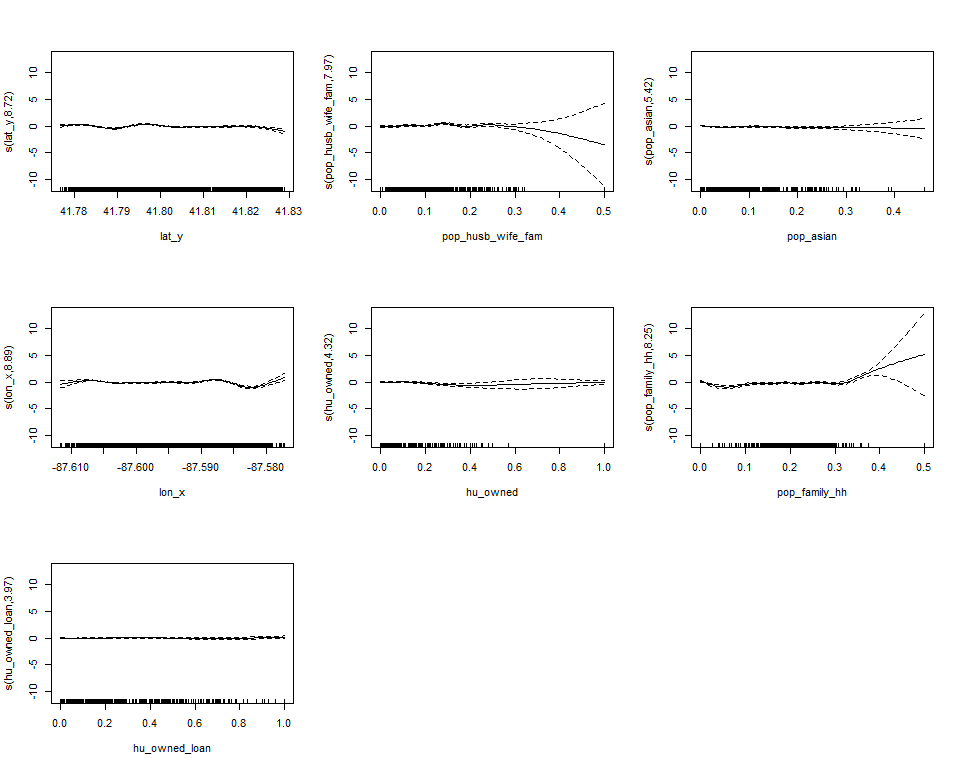
\includegraphics[width=1\textwidth,height=\textheight]{..//Modeling/modeling_files/figure-gfm/gam-arrests-1.png}
\caption{Arrest Model - Plots of Nonlinear GAM Covariates}
\end{figure}

Similarly, the most significant coefficients in the GAM model are
primarily types of violent crimes. Interference with a public officer
has a predicted 92\% chance of ending in arrest. Crimes involving
narcotics have a similarly high 94\% chance. Interestingly, crimes where
the suspect was reported as being armed have a very low probability of
ending in arrest, at 4\%. This appears to indicate that instigators of
weapons violations are less likely to be apprehended following the
crime. While the nonlinear terms are all highly significant, except for
proportion of one person households, none of them have a very strong
relationship with the dependent variable. This model had a ROC AUC of
0.839, indicating good predictive performance.

\hypertarget{responding-department}{%
\subsection{Responding Department}\label{responding-department}}

\hypertarget{ucpd-versus-cpd}{%
\subsubsection{UCPD Versus CPD}\label{ucpd-versus-cpd}}

\begin{table}

\caption{\label{tab:ucpd-lasso}UCPD vs. CPD Model Coefficient Estimates - Lasso Regression}
\centering
\begin{tabular}[t]{l|r}
\hline
Variable & Est.\\
\hline
(Intercept) & -3543.027\\
\hline
lon\_x & -64.122\\
\hline
lat\_y & -49.665\\
\hline
pop\_family\_hh & -4.773\\
\hline
pop\_asian & 3.659\\
\hline
primary\_type.liquor law violation & 3.474\\
\hline
primary\_type.harassment & 2.113\\
\hline
pop\_white & 1.852\\
\hline
domestic.TRUE & -1.579\\
\hline
primary\_type.other & 1.484\\
\hline
pop\_latino & 1.300\\
\hline
primary\_type.deceptive practice & -1.069\\
\hline
pop\_black & -1.004\\
\hline
primary\_type.assault & -0.617\\
\hline
pop\_in\_hus & -0.490\\
\hline
primary\_type.public peace violation & 0.407\\
\hline
pop\_one\_pers\_hh & 0.368\\
\hline
aggravated.TRUE & -0.287\\
\hline
primary\_type.theft & 0.272\\
\hline
primary\_type.sex crime & -0.218\\
\hline
primary\_type.narcotics & -0.217\\
\hline
primary\_type.battery & -0.182\\
\hline
hu\_vacant & -0.107\\
\hline
month.jun & -0.093\\
\hline
month.dec & -0.056\\
\hline
month.nov & 0.052\\
\hline
avg\_family\_size & -0.036\\
\hline
avg\_household\_size & -0.030\\
\hline
weekend.TRUE & -0.027\\
\hline
month.oct & 0.002\\
\hline
date & 0.000\\
\hline
\end{tabular}
\end{table}

From this lasso regression model, it appears the UCPD is less likely to
respond to incidents to the north and west, in areas where there are
more families and blacks, and to domestic crimes. However, it appears
that officers from the university are more likely to respond to crimes
reported where there is a higher proportion of any other race than
black, and to crimes involving liquor law violations and harassment.
This model had a ROC AUC of 0.872, indicating good predictive
performance.

\begin{table}

\caption{\label{tab:ucpd-gam}UCPD vs. CPD Linear Coefficient Estimates - GAM}
\centering
\begin{tabular}[t]{l|r|r|r|r}
\hline
Variable & Est. & Std. Error & Z Value & P Value\\
\hline
(Intercept) & -3.667 & 1.225 & -2.992 & 0.003\\
\hline
primary\_typeassault & -1.299 & 0.961 & -1.351 & 0.177\\
\hline
primary\_typebattery & -0.572 & 0.955 & -0.599 & 0.549\\
\hline
primary\_typeburglary & -0.678 & 0.956 & -0.709 & 0.478\\
\hline
primary\_typedamage & -0.632 & 0.954 & -0.662 & 0.508\\
\hline
primary\_typedeceptive practice & -2.483 & 0.966 & -2.571 & 0.010\\
\hline
primary\_typeharassment & 1.914 & 1.001 & 1.912 & 0.056\\
\hline
primary\_typehomicide & -85.991 & 11032629.281 & 0.000 & 1.000\\
\hline
primary\_typeinterference with public officer & -0.079 & 1.130 & -0.070 & 0.944\\
\hline
primary\_typeliquor law violation & 3.951 & 1.017 & 3.884 & 0.000\\
\hline
primary\_typenarcotics & -0.061 & 0.959 & -0.063 & 0.949\\
\hline
primary\_typeother & 1.098 & 0.953 & 1.152 & 0.250\\
\hline
primary\_typepublic peace violation & 1.118 & 0.971 & 1.151 & 0.250\\
\hline
primary\_typerobbery & -0.089 & 0.957 & -0.093 & 0.926\\
\hline
primary\_typesex crime & -2.092 & 0.994 & -2.105 & 0.035\\
\hline
primary\_typetheft & -0.599 & 0.952 & -0.629 & 0.530\\
\hline
primary\_typetrespassing & -0.337 & 0.961 & -0.351 & 0.725\\
\hline
primary\_typeweapons violation & 0.239 & 0.982 & 0.243 & 0.808\\
\hline
domesticTRUE & -2.337 & 0.141 & -16.522 & 0.000\\
\hline
\end{tabular}
\end{table}

\begin{table}

\caption{\label{tab:ucpd-gam}UCPD vs. CPD Smooth Coefficient Estimates - GAM}
\centering
\begin{tabular}[t]{l|r|r|r}
\hline
Variable & Est. Df & Chi Sq. & P Value\\
\hline
s(lon\_x) & 8.812 & 1214.799 & 0\\
\hline
s(lat\_y) & 8.085 & 1803.070 & 0\\
\hline
s(pop\_family\_hh) & 8.300 & 98.541 & 0\\
\hline
s(pop\_asian) & 8.386 & 64.780 & 0\\
\hline
s(pop\_white) & 8.722 & 36.337 & 0\\
\hline
s(pop\_latino) & 8.000 & 106.972 & 0\\
\hline
s(pop\_black) & 8.642 & 75.161 & 0\\
\hline
s(pop\_in\_hus) & 8.908 & 100.549 & 0\\
\hline
\end{tabular}
\end{table}

\begin{figure}
\centering
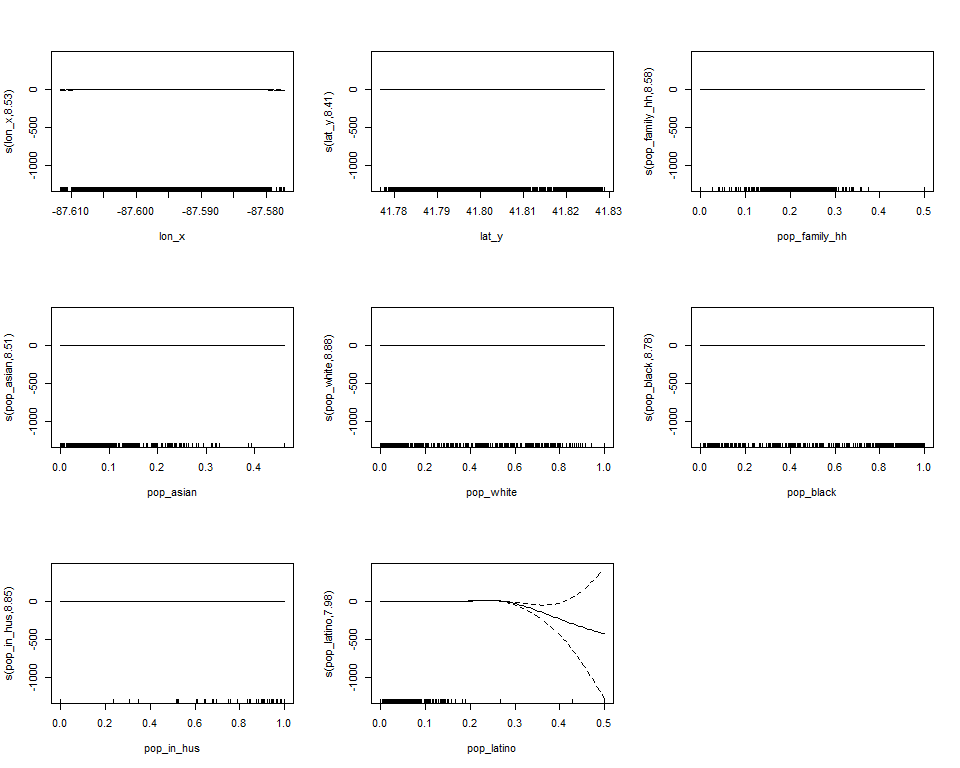
\includegraphics[width=1\textwidth,height=\textheight]{..//Modeling/modeling_files/figure-gfm/gam-ucpd-1.png}
\caption{UCPD vs.~CPD - Plots of Nonlinear GAM Covariates}
\end{figure}

The estimates from the lasso closely match those from the GAM model.
Crimes reported to have involved a domestic incident, liquor law
violation, and deceptive practice are all significant. There is an
estimated 57\% probability of UCPD responding to a liquor law violation,
estimated 0\% probability of responding to an incident of deceptive
practice, and a 0\% chance of responding to a domestic incident. While
the nonlinear terms are all highly significant, none of them have a very
strong relationship with the dependent variable. This model had a ROC
AUC of 0.869, indicating good predictive performance.

\hypertarget{both-departments-versus-each-department}{%
\subsubsection{Both Departments Versus Each
Department}\label{both-departments-versus-each-department}}

\begin{table}

\caption{\label{tab:both-lasso}Both vs. Each Model Coefficient Estimates - Lasso Regression}
\centering
\begin{tabular}[t]{l|r}
\hline
Variable & Est.\\
\hline
(Intercept) & 1443.750\\
\hline
lat\_y & -21.004\\
\hline
lon\_x & 6.651\\
\hline
primary\_type.homicide & 4.525\\
\hline
primary\_type.robbery & 2.781\\
\hline
pop\_latino & 1.954\\
\hline
domestic.TRUE & -1.942\\
\hline
primary\_type.burglary & 1.734\\
\hline
primary\_type.other & 1.679\\
\hline
primary\_type.deceptive practice & -1.375\\
\hline
primary\_type.weapons violation & 1.208\\
\hline
aggravated.TRUE & 1.193\\
\hline
pop\_asian & 1.124\\
\hline
primary\_type.liquor law violation & -1.047\\
\hline
pop\_black & -1.045\\
\hline
hu\_owned & 1.033\\
\hline
primary\_type.sex crime & 0.997\\
\hline
primary\_type.battery & 0.607\\
\hline
pop\_white & 0.592\\
\hline
pop\_family\_hh & -0.513\\
\hline
arrest.TRUE & -0.494\\
\hline
pop\_in\_hus & 0.394\\
\hline
primary\_type.theft & -0.342\\
\hline
primary\_type.damage & -0.327\\
\hline
hu\_rented & 0.275\\
\hline
armed.TRUE & 0.218\\
\hline
avg\_family\_size & 0.153\\
\hline
month.feb & -0.144\\
\hline
day\_of\_week.sat & 0.120\\
\hline
month.jun & 0.085\\
\hline
day\_of\_week.tue & 0.074\\
\hline
hu\_owned\_loan & 0.073\\
\hline
hu\_vacant & -0.040\\
\hline
day\_of\_week.mon & -0.036\\
\hline
month.oct & 0.024\\
\hline
pop\_one\_pers\_hh & 0.016\\
\hline
time & 0.008\\
\hline
month.dec & -0.001\\
\hline
date & 0.000\\
\hline
\end{tabular}
\end{table}

The lasso regression model indicates that both departments are less
likely to respond to crimes toward the south and east, crimes located in
areas with higher proportions of blacks, and crimes involving domestic
incidents, deceptive practice, or liquor law violations. However, both
departments are more likely to respond to reported crimes involving
homicide, robbery, and to a lesser degree burglary and weapons
violations. Crimes that were reported to have occurred in areas with
higher populations of Asians or Latinos are also more likely to have
both departments respond. This model had a ROC AUC of 0.836, indicating
good predictive performance.

\begin{table}

\caption{\label{tab:both-gam}Both vs. Each Linear Coefficient Estimates - GAM}
\centering
\begin{tabular}[t]{l|r|r|r|r}
\hline
Variable & Est. & Std. Error & Z Value & P Value\\
\hline
(Intercept) & -143.060 & 11863283.204 & 0.000 & 1\\
\hline
primary\_typeassault & 138.273 & 11863283.204 & 0.000 & 1\\
\hline
primary\_typebattery & 139.054 & 11863283.204 & 0.000 & 1\\
\hline
primary\_typeburglary & 139.823 & 11863283.204 & 0.000 & 1\\
\hline
primary\_typedamage & 137.634 & 11863283.204 & 0.000 & 1\\
\hline
primary\_typedeceptive practice & 135.880 & 11863283.204 & 0.000 & 1\\
\hline
primary\_typeharassment & 137.862 & 11863283.204 & 0.000 & 1\\
\hline
primary\_typehomicide & 142.977 & 11863283.204 & 0.000 & 1\\
\hline
primary\_typeinterference with public officer & 103.806 & 14169879.447 & 0.000 & 1\\
\hline
primary\_typeliquor law violation & 102.909 & 12479963.403 & 0.000 & 1\\
\hline
primary\_typenarcotics & 136.128 & 11863283.204 & 0.000 & 1\\
\hline
primary\_typeother & 139.918 & 11863283.204 & 0.000 & 1\\
\hline
primary\_typepublic peace violation & 138.072 & 11863283.204 & 0.000 & 1\\
\hline
primary\_typerobbery & 141.095 & 11863283.204 & 0.000 & 1\\
\hline
primary\_typesex crime & 139.454 & 11863283.204 & 0.000 & 1\\
\hline
primary\_typetheft & 137.688 & 11863283.204 & 0.000 & 1\\
\hline
primary\_typetrespassing & 138.281 & 11863283.204 & 0.000 & 1\\
\hline
primary\_typeweapons violation & 139.712 & 11863283.204 & 0.000 & 1\\
\hline
domesticTRUE & -2.506 & 0.243 & -10.312 & 0\\
\hline
aggravatedTRUE & 1.151 & 0.102 & 11.330 & 0\\
\hline
\end{tabular}
\end{table}

\begin{table}

\caption{\label{tab:both-gam}Both vs. Each Smooth Coefficient Estimates - GAM}
\centering
\begin{tabular}[t]{l|r|r|r}
\hline
Variable & Est. Df & Chi Sq. & P Value\\
\hline
s(lat\_y) & 6.715 & 193.487 & 0.000\\
\hline
s(lon\_x) & 8.916 & 79.787 & 0.000\\
\hline
s(pop\_latino) & 1.148 & 1.451 & 0.218\\
\hline
s(pop\_asian) & 1.002 & 0.091 & 0.764\\
\hline
s(pop\_black) & 1.000 & 0.010 & 0.922\\
\hline
s(hu\_owned) & 5.221 & 26.383 & 0.000\\
\hline
s(pop\_white) & 7.145 & 23.967 & 0.003\\
\hline
\end{tabular}
\end{table}

\begin{figure}
\centering
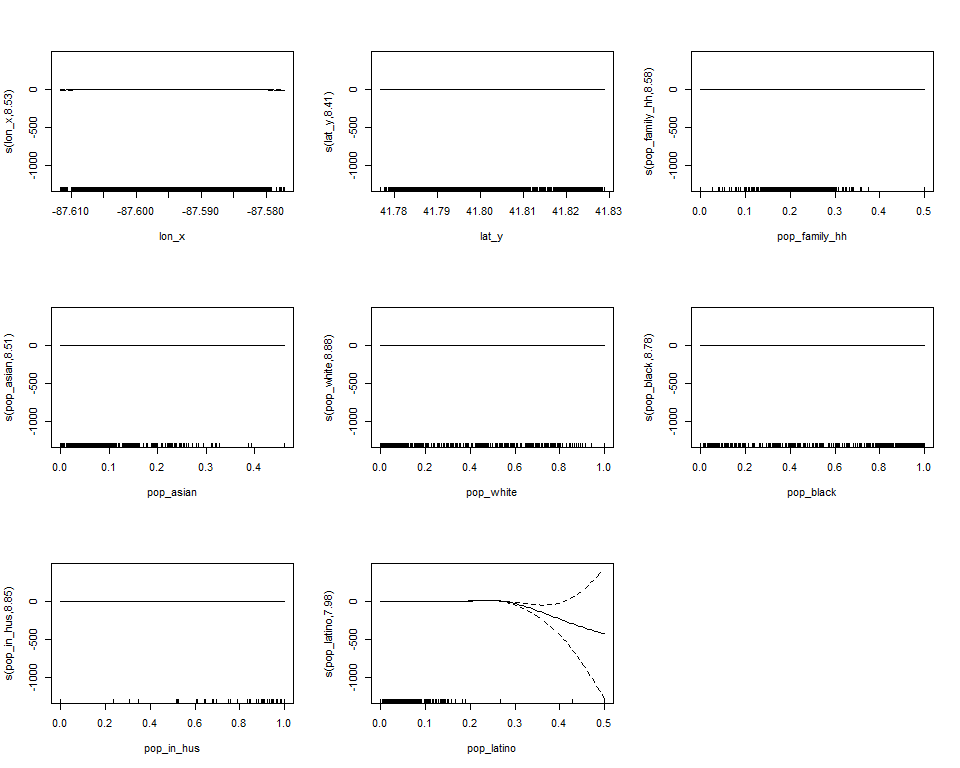
\includegraphics[width=1\textwidth,height=\textheight]{..//Modeling/modeling_files/figure-gfm/gam-both-1.png}
\caption{Both vs.~Each - Plots of Nonlinear GAM Covariates}
\end{figure}

However, while the GAM model had a ROC AUC of 0.742, indicating good
predictive performance, it appears that this model is not very accurate.
Many of the linear estimates for this GAM model are wildly large and
highly insignificant. This could be due, in part, to a number of
variables specified as non-linear terms that should be linear terms. The
smooth estimates for proportion Asian and proportion black both have
estimated degrees of freedom close to 1, indicating they should be
linear terms, not non-linear terms. While the nonlinear terms are all
highly significant, except for proportion black, Asian, and Latino, none
of them have a very strong relationship with the dependent variable.

\hypertarget{race}{%
\subsection{Race}\label{race}}

\begin{table}

\caption{\label{tab:asian-lasso}Asian Model Coefficient Estimates - Lasso Regression}
\centering
\begin{tabular}[t]{l|r}
\hline
Variable & Est.\\
\hline
(Intercept) & -9.264\\
\hline
lat\_y & -0.309\\
\hline
lon\_x & -0.253\\
\hline
pop\_female & 0.168\\
\hline
pop\_family\_hh & -0.157\\
\hline
pop\_black & -0.133\\
\hline
pop\_husb\_wife\_fam & 0.088\\
\hline
pop\_one\_pers\_hh & 0.077\\
\hline
hu\_owned & 0.058\\
\hline
pop\_under\_18 & -0.048\\
\hline
hu\_owned\_loan & 0.042\\
\hline
pop\_in\_hus & 0.029\\
\hline
hu\_rented & 0.027\\
\hline
avg\_family\_size & 0.009\\
\hline
responding\_dept.ucpd & 0.006\\
\hline
pop\_white & -0.006\\
\hline
primary\_type.liquor law violation & 0.005\\
\hline
responding\_dept.cpd & -0.003\\
\hline
arrest.TRUE & -0.003\\
\hline
primary\_type.battery & -0.002\\
\hline
primary\_type.damage & 0.002\\
\hline
attempted.TRUE & 0.002\\
\hline
avg\_household\_size & -0.002\\
\hline
primary\_type.assault & -0.001\\
\hline
primary\_type.burglary & 0.001\\
\hline
primary\_type.harassment & 0.001\\
\hline
primary\_type.interference with public officer & 0.001\\
\hline
primary\_type.public peace violation & -0.001\\
\hline
primary\_type.robbery & 0.001\\
\hline
primary\_type.theft & 0.001\\
\hline
month.mar & -0.001\\
\hline
median\_age & -0.001\\
\hline
primary\_type.other & 0.000\\
\hline
time & 0.000\\
\hline
weekend.TRUE & 0.000\\
\hline
total\_housing\_units & 0.000\\
\hline
hu\_vacant & 0.000\\
\hline
total\_pop & 0.000\\
\hline
pop\_latino & 0.000\\
\hline
\end{tabular}
\end{table}

\begin{table}

\caption{\label{tab:asian-gam}Asian Linear Coefficient Estimates - GAM}
\centering
\begin{tabular}[t]{l|r|r|r|r}
\hline
Variable & Est. & Std. Error & Z Value & P Value\\
\hline
(Intercept) & 0.039 & 0.004 & 8.678 & 0.000\\
\hline
responding\_deptcpd & 0.000 & 0.001 & 0.478 & 0.633\\
\hline
responding\_deptucpd & -0.003 & 0.001 & -3.991 & 0.000\\
\hline
primary\_typeassault & 0.002 & 0.004 & 0.450 & 0.652\\
\hline
primary\_typebattery & 0.002 & 0.004 & 0.556 & 0.579\\
\hline
primary\_typeburglary & 0.005 & 0.004 & 1.027 & 0.304\\
\hline
primary\_typedamage & 0.004 & 0.004 & 0.887 & 0.375\\
\hline
primary\_typedeceptive practice & 0.004 & 0.004 & 0.923 & 0.356\\
\hline
primary\_typeharassment & 0.006 & 0.005 & 1.257 & 0.209\\
\hline
primary\_typehomicide & 0.001 & 0.006 & 0.240 & 0.810\\
\hline
primary\_typeinterference with public officer & 0.006 & 0.005 & 1.223 & 0.221\\
\hline
primary\_typeliquor law violation & 0.006 & 0.005 & 1.297 & 0.195\\
\hline
primary\_typenarcotics & 0.002 & 0.004 & 0.428 & 0.669\\
\hline
primary\_typeother & 0.003 & 0.004 & 0.570 & 0.568\\
\hline
primary\_typepublic peace violation & 0.003 & 0.005 & 0.693 & 0.488\\
\hline
primary\_typerobbery & 0.003 & 0.004 & 0.752 & 0.452\\
\hline
primary\_typesex crime & 0.001 & 0.005 & 0.296 & 0.767\\
\hline
primary\_typetheft & 0.003 & 0.004 & 0.714 & 0.475\\
\hline
primary\_typetrespassing & 0.002 & 0.004 & 0.402 & 0.688\\
\hline
primary\_typeweapons violation & 0.003 & 0.005 & 0.600 & 0.549\\
\hline
arrestTRUE & 0.000 & 0.000 & -0.522 & 0.602\\
\hline
attemptedTRUE & 0.002 & 0.001 & 1.680 & 0.093\\
\hline
monthfeb & 0.000 & 0.001 & 0.733 & 0.464\\
\hline
monthmar & 0.000 & 0.001 & -0.623 & 0.533\\
\hline
monthapr & 0.000 & 0.001 & 0.492 & 0.623\\
\hline
monthmay & 0.000 & 0.001 & 0.078 & 0.938\\
\hline
monthjun & 0.000 & 0.001 & 0.431 & 0.666\\
\hline
monthjul & 0.000 & 0.001 & 0.791 & 0.429\\
\hline
monthaug & 0.001 & 0.001 & 1.646 & 0.100\\
\hline
monthsep & 0.000 & 0.001 & -0.601 & 0.548\\
\hline
monthoct & 0.000 & 0.001 & 0.495 & 0.621\\
\hline
monthnov & 0.000 & 0.001 & 0.862 & 0.389\\
\hline
monthdec & 0.000 & 0.001 & 0.474 & 0.636\\
\hline
\end{tabular}
\end{table}

\begin{table}

\caption{\label{tab:asian-gam}Asian Smooth Coefficient Estimates - GAM}
\centering
\begin{tabular}[t]{l|r|r|r}
\hline
Variable & Est. Df & Chi Sq. & P Value\\
\hline
s(lat\_y) & 8.989 & 2156.164 & 0\\
\hline
s(lon\_x) & 8.988 & 1410.353 & 0\\
\hline
s(pop\_female) & 8.994 & 14032.740 & 0\\
\hline
s(pop\_family\_hh) & 9.000 & 1175.940 & 0\\
\hline
s(pop\_black) & 9.000 & 18758.123 & 0\\
\hline
s(pop\_husb\_wife\_fam) & 8.954 & 1822.599 & 0\\
\hline
s(pop\_one\_pers\_hh) & 8.975 & 3024.511 & 0\\
\hline
s(hu\_owned) & 8.983 & 2331.405 & 0\\
\hline
s(pop\_under\_18) & 8.967 & 760.068 & 0\\
\hline
s(hu\_owned\_loan) & 8.999 & 2070.522 & 0\\
\hline
s(pop\_in\_hus) & 8.995 & 3010.942 & 0\\
\hline
s(hu\_rented) & 8.981 & 1696.386 & 0\\
\hline
s(avg\_family\_size) & 8.992 & 2410.041 & 0\\
\hline
s(pop\_white) & 8.995 & 19489.786 & 0\\
\hline
s(avg\_household\_size) & 8.999 & 3071.478 & 0\\
\hline
\end{tabular}
\end{table}

\begin{figure}
\centering
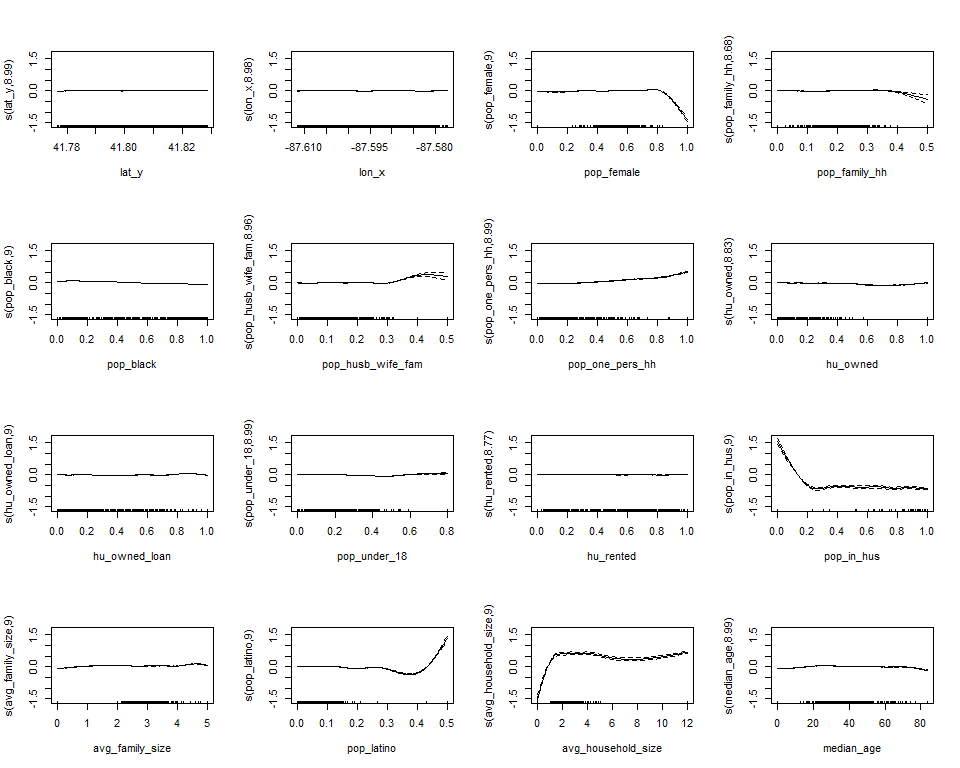
\includegraphics[width=1\textwidth,height=\textheight]{..//Modeling/modeling_files/figure-gfm/gam-asian-1.png}
\caption{Asian Model - Plots of Nonlinear GAM Covariates}
\end{figure}

\begin{table}

\caption{\label{tab:black-lasso}Black Model Coefficient Estimates - Lasso Regression}
\centering
\begin{tabular}[t]{l|r}
\hline
Variable & Est.\\
\hline
(Intercept) & -139.691\\
\hline
lon\_x & -1.595\\
\hline
pop\_husb\_wife\_fam & -0.781\\
\hline
pop\_white & -0.702\\
\hline
pop\_asian & -0.679\\
\hline
pop\_female & 0.432\\
\hline
pop\_under\_18 & 0.411\\
\hline
pop\_in\_hus & 0.171\\
\hline
pop\_family\_hh & 0.049\\
\hline
hu\_vacant & 0.041\\
\hline
hu\_rented & 0.031\\
\hline
avg\_family\_size & 0.029\\
\hline
primary\_type.liquor law violation & 0.012\\
\hline
median\_age & 0.008\\
\hline
avg\_household\_size & 0.004\\
\hline
primary\_type.damage & 0.001\\
\hline
hu\_owned & -0.001\\
\hline
responding\_dept.ucpd & 0.000\\
\hline
primary\_type.robbery & 0.000\\
\hline
total\_housing\_units & 0.000\\
\hline
total\_pop & 0.000\\
\hline
\end{tabular}
\end{table}

\begin{table}

\caption{\label{tab:black-gam}Black Linear Coefficient Estimates - GAM}
\centering
\begin{tabular}[t]{l|r|r|r|r}
\hline
Variable & Est. & Std. Error & Z Value & P Value\\
\hline
(Intercept) & 0.473 & 0.004 & 125.550 & 0.000\\
\hline
primary\_typeassault & -0.003 & 0.004 & -0.812 & 0.417\\
\hline
primary\_typebattery & -0.003 & 0.004 & -0.757 & 0.449\\
\hline
primary\_typeburglary & -0.002 & 0.004 & -0.516 & 0.606\\
\hline
primary\_typedamage & -0.001 & 0.004 & -0.367 & 0.713\\
\hline
primary\_typedeceptive practice & -0.004 & 0.004 & -1.190 & 0.234\\
\hline
primary\_typeharassment & -0.002 & 0.004 & -0.454 & 0.650\\
\hline
primary\_typehomicide & -0.008 & 0.005 & -1.713 & 0.087\\
\hline
primary\_typeinterference with public officer & -0.003 & 0.004 & -0.611 & 0.541\\
\hline
primary\_typeliquor law violation & -0.004 & 0.004 & -0.969 & 0.333\\
\hline
primary\_typenarcotics & -0.004 & 0.004 & -0.964 & 0.335\\
\hline
primary\_typeother & -0.002 & 0.004 & -0.579 & 0.563\\
\hline
primary\_typepublic peace violation & -0.003 & 0.004 & -0.746 & 0.456\\
\hline
primary\_typerobbery & -0.005 & 0.004 & -1.284 & 0.199\\
\hline
primary\_typesex crime & -0.004 & 0.004 & -0.998 & 0.318\\
\hline
primary\_typetheft & -0.003 & 0.004 & -0.779 & 0.436\\
\hline
primary\_typetrespassing & -0.003 & 0.004 & -0.690 & 0.490\\
\hline
primary\_typeweapons violation & -0.003 & 0.004 & -0.748 & 0.454\\
\hline
responding\_deptcpd & 0.000 & 0.001 & -0.859 & 0.390\\
\hline
responding\_deptucpd & -0.002 & 0.001 & -2.907 & 0.004\\
\hline
\end{tabular}
\end{table}

\begin{table}

\caption{\label{tab:black-gam}Black Smooth Coefficient Estimates - GAM}
\centering
\begin{tabular}[t]{l|r|r|r}
\hline
Variable & Est. Df & Chi Sq. & P Value\\
\hline
s(lon\_x) & 8.802 & 941.665 & 0\\
\hline
s(pop\_husb\_wife\_fam) & 9.000 & 1743.744 & 0\\
\hline
s(pop\_white) & 8.987 & 450051.920 & 0\\
\hline
s(pop\_asian) & 8.995 & 78584.357 & 0\\
\hline
s(pop\_female) & 9.000 & 4841.490 & 0\\
\hline
s(pop\_under\_18) & 9.000 & 5669.525 & 0\\
\hline
s(pop\_in\_hus) & 8.994 & 1204.399 & 0\\
\hline
s(pop\_family\_hh) & 9.000 & 1647.345 & 0\\
\hline
s(hu\_vacant) & 8.989 & 5133.575 & 0\\
\hline
s(hu\_rented) & 8.995 & 3717.724 & 0\\
\hline
s(avg\_family\_size) & 8.994 & 3369.513 & 0\\
\hline
s(median\_age) & 8.994 & 393682.436 & 0\\
\hline
s(avg\_household\_size) & 8.986 & 3180.626 & 0\\
\hline
s(hu\_owned) & 8.991 & 2646.879 & 0\\
\hline
s(total\_housing\_units) & 9.000 & 1937.170 & 0\\
\hline
s(total\_pop) & 9.000 & 1532.429 & 0\\
\hline
\end{tabular}
\end{table}

\begin{figure}
\centering
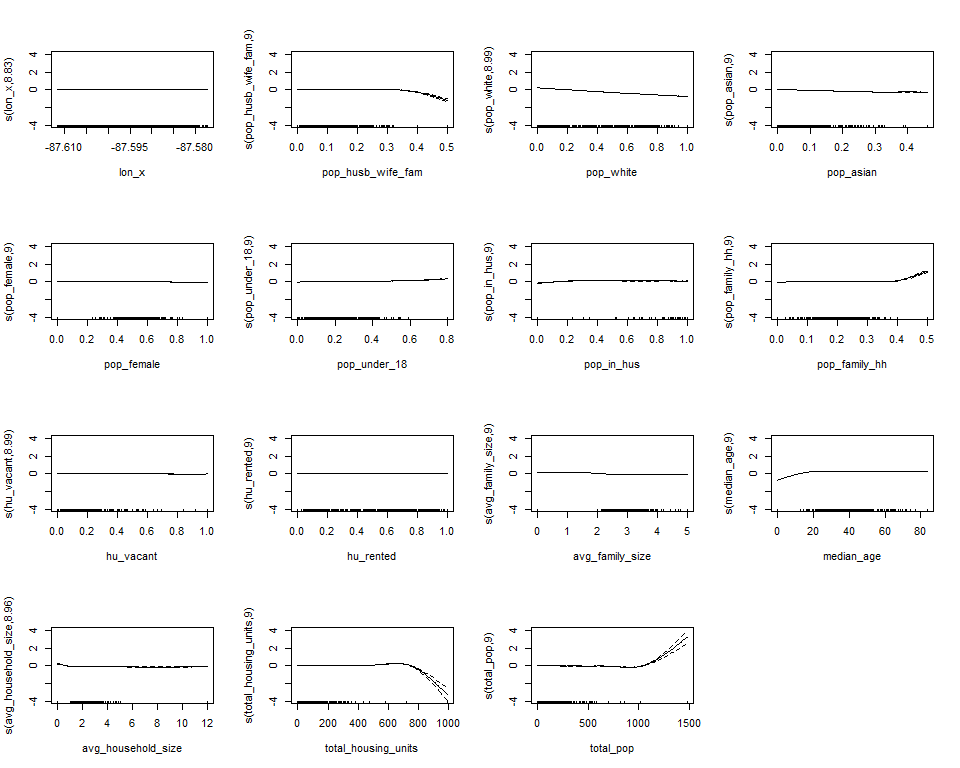
\includegraphics[width=1\textwidth,height=\textheight]{..//Modeling/modeling_files/figure-gfm/gam-black-1.png}
\caption{Black Model - Plots of Nonlinear GAM Covariates}
\end{figure}

\begin{table}

\caption{\label{tab:white-lasso}White Model Coefficient Estimates - Lasso Regression}
\centering
\begin{tabular}[t]{l|r}
\hline
Variable & Est.\\
\hline
(Intercept) & 18.617\\
\hline
pop\_black & -0.719\\
\hline
pop\_female & 0.570\\
\hline
pop\_latino & 0.416\\
\hline
pop\_husb\_wife\_fam & 0.289\\
\hline
pop\_family\_hh & -0.261\\
\hline
lat\_y & -0.251\\
\hline
pop\_in\_hus & 0.158\\
\hline
hu\_owned & 0.149\\
\hline
pop\_one\_pers\_hh & -0.110\\
\hline
hu\_owned\_loan & -0.105\\
\hline
lon\_x & 0.089\\
\hline
hu\_vacant & 0.067\\
\hline
pop\_under\_18 & -0.067\\
\hline
avg\_household\_size & 0.041\\
\hline
pop\_asian & -0.021\\
\hline
responding\_dept.ucpd & 0.019\\
\hline
responding\_dept.cpd & -0.014\\
\hline
primary\_type.narcotics & -0.013\\
\hline
primary\_type.liquor law violation & 0.009\\
\hline
primary\_type.burglary & 0.008\\
\hline
median\_age & 0.006\\
\hline
primary\_type.weapons violation & -0.005\\
\hline
hu\_rented & 0.005\\
\hline
primary\_type.interference with public officer & -0.004\\
\hline
avg\_family\_size & -0.002\\
\hline
primary\_type.assault & -0.001\\
\hline
primary\_type.battery & -0.001\\
\hline
arrest.TRUE & -0.001\\
\hline
month.aug & -0.001\\
\hline
primary\_type.harassment & 0.000\\
\hline
primary\_type.robbery & 0.000\\
\hline
primary\_type.theft & 0.000\\
\hline
month.apr & 0.000\\
\hline
month.oct & 0.000\\
\hline
year & 0.000\\
\hline
total\_housing\_units & 0.000\\
\hline
total\_pop & 0.000\\
\hline
\end{tabular}
\end{table}

\begin{table}

\caption{\label{tab:white-gam}White Linear Coefficient Estimates - GAM}
\centering
\begin{tabular}[t]{l|r|r|r|r}
\hline
Variable & Est. & Std. Error & Z Value & P Value\\
\hline
(Intercept) & 0.204 & 0.003 & 75.507 & 0.000\\
\hline
responding\_deptcpd & -0.001 & 0.000 & -1.941 & 0.052\\
\hline
responding\_deptucpd & 0.000 & 0.000 & 0.354 & 0.723\\
\hline
primary\_typeassault & -0.004 & 0.003 & -1.317 & 0.188\\
\hline
primary\_typebattery & -0.003 & 0.003 & -1.284 & 0.199\\
\hline
primary\_typeburglary & -0.004 & 0.003 & -1.350 & 0.177\\
\hline
primary\_typedamage & -0.003 & 0.003 & -1.127 & 0.260\\
\hline
primary\_typedeceptive practice & -0.004 & 0.003 & -1.523 & 0.128\\
\hline
primary\_typeharassment & -0.004 & 0.003 & -1.280 & 0.201\\
\hline
primary\_typehomicide & -0.010 & 0.003 & -2.992 & 0.003\\
\hline
primary\_typeinterference with public officer & -0.007 & 0.003 & -2.051 & 0.040\\
\hline
primary\_typeliquor law violation & -0.007 & 0.003 & -2.474 & 0.013\\
\hline
primary\_typenarcotics & -0.004 & 0.003 & -1.659 & 0.097\\
\hline
primary\_typeother & -0.004 & 0.003 & -1.344 & 0.179\\
\hline
primary\_typepublic peace violation & -0.004 & 0.003 & -1.398 & 0.162\\
\hline
primary\_typerobbery & -0.004 & 0.003 & -1.602 & 0.109\\
\hline
primary\_typesex crime & -0.003 & 0.003 & -1.058 & 0.290\\
\hline
primary\_typetheft & -0.004 & 0.003 & -1.317 & 0.188\\
\hline
primary\_typetrespassing & -0.004 & 0.003 & -1.514 & 0.130\\
\hline
primary\_typeweapons violation & -0.004 & 0.003 & -1.529 & 0.126\\
\hline
\end{tabular}
\end{table}

\begin{table}

\caption{\label{tab:white-gam}White Smooth Coefficient Estimates - GAM}
\centering
\begin{tabular}[t]{l|r|r|r}
\hline
Variable & Est. Df & Chi Sq. & P Value\\
\hline
s(pop\_black) & 8.984 & 683578.889 & 0\\
\hline
s(pop\_female) & 9.000 & 6720.006 & 0\\
\hline
s(pop\_latino) & 8.998 & 14533.160 & 0\\
\hline
s(pop\_husb\_wife\_fam) & 8.933 & 1388.254 & 0\\
\hline
s(pop\_family\_hh) & 8.978 & 781.874 & 0\\
\hline
s(lat\_y) & 8.977 & 1918.108 & 0\\
\hline
s(pop\_in\_hus) & 9.000 & 1546.135 & 0\\
\hline
s(hu\_owned) & 8.984 & 1542.512 & 0\\
\hline
s(pop\_one\_pers\_hh) & 8.995 & 3480.792 & 0\\
\hline
s(hu\_owned\_loan) & 8.991 & 2887.830 & 0\\
\hline
s(lon\_x) & 8.988 & 1881.473 & 0\\
\hline
s(hu\_vacant) & 9.000 & 3364.801 & 0\\
\hline
s(pop\_under\_18) & 9.000 & 4482.106 & 0\\
\hline
s(avg\_household\_size) & 8.554 & 3021.173 & 0\\
\hline
s(pop\_asian) & 8.806 & 131339.315 & 0\\
\hline
s(median\_age) & 9.000 & 269867.070 & 0\\
\hline
s(hu\_rented) & 8.994 & 5282.521 & 0\\
\hline
s(avg\_family\_size) & 8.983 & 1321.425 & 0\\
\hline
\end{tabular}
\end{table}

\begin{figure}
\centering
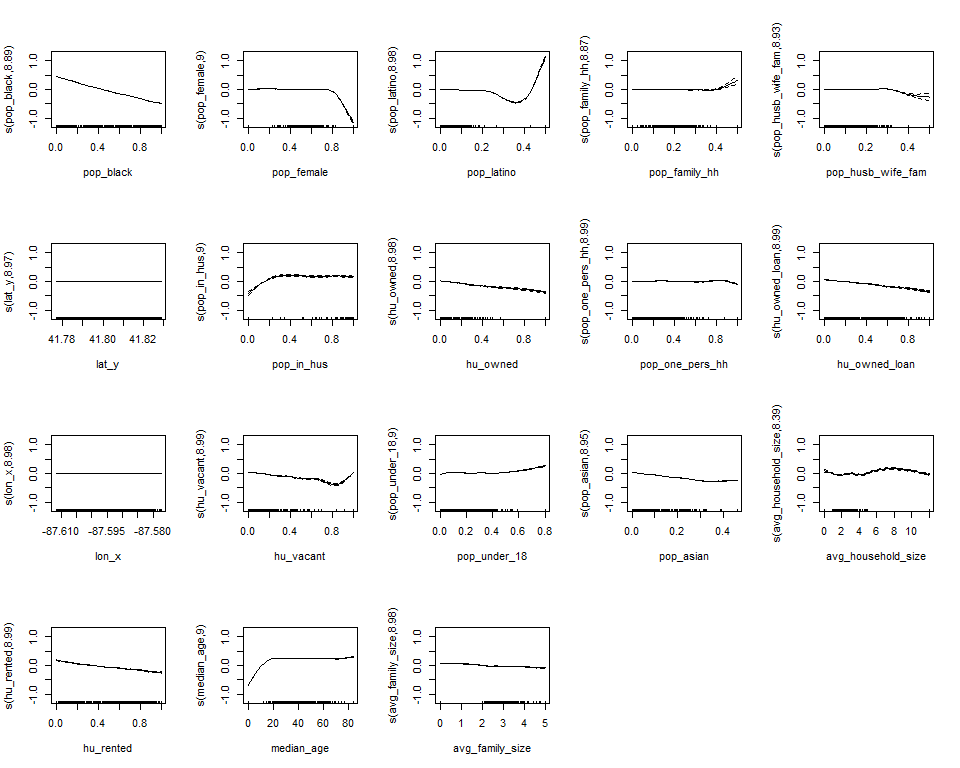
\includegraphics[width=1\textwidth,height=\textheight]{..//Modeling/modeling_files/figure-gfm/gam-white-1.png}
\caption{White Model - Plots of Nonlinear GAM Covariates}
\end{figure}

\begin{table}

\caption{\label{tab:race-performance}Performance of Race Models}
\centering
\begin{tabular}[t]{l|r}
\hline
Model & RMSE\\
\hline
Asian Lasso & 0.038\\
\hline
Asian GAM & 0.025\\
\hline
Black Lasso & 0.086\\
\hline
Black GAM & 0.020\\
\hline
White Lasso & 0.087\\
\hline
White GAM & 0.016\\
\hline
\end{tabular}
\end{table}

When predicting racial makeup of an area where a crime occurred, it
appears that other demographic variables account for most of the
variation in the outcome. Proportion Asian and black both have a
significant negative relationship with the responding department being
UCPD. However, this accompanies only a small change of a few tenths of a
percentage less of each race in the areas where UCPD responds to
reported crimes. For the proportion of whites, the only significant
relationships are with the reported crime type being homicide or
interference with a public officer. Both account for approximately 1\%
less white people in the areas where those types of crimes occur.

\hypertarget{discussion}{%
\chapter{Discussion}\label{discussion}}

It is clear that the actions of each department reflect the community
for which they are policing. The UCPD is more likely to respond to a
liquor law violation, but much less likely to make an arrest for it.
While the UCPD handles an equivalent proportion of crimes involving
narcotics as the CPD, they proportionally also made much fewer arrests.
While both departments handle a large amount of thefts on their own,
UCPD responds to a larger proportion of theft, and many other incidents
such as missing property where a crime may have occurred. It appears
that the UCPD does try to fit this ``parental'' role as referenced by
Williams et al. (2016). Instead of being excessively punitive, as they
could for petty crimes like liquor law violations, they appear to simply
respond and nothing more in the vast majority of cases. Likely campus
officers are administering verbal warnings for crimes like under-aged
drinking, that university students are likely to engage in, but pose
little threat to other community members.

However, there are some cases where UCPD officers appear to be equally
or more punitive than their city counterparts. Officers from either
department are highly likely to make an arrest when someone is
interfering in their policing activities. Furthermore, when campus
police respond to crimes of trespassing or sex crimes there is a higher
likelihood of an arrest being made. Again, this seems to be indicative
of differences in the communities each department polices. Especially at
a private university, there are many amenities only accessible to the
university community, and not the public at large. University officers
may be more likely to punish people who are not affiliated with the
university, trespassing on private university property, to reinforce the
exclusivity of those spaces. Additionally, University members are
unlikely to be sympathetic to these trespassers, who students and
faculty are likely to see as taking resources that outsiders are not
entitled to.

Sex crimes could be a similar situation, where stakeholders in the
community view the issue as one warranting more putative measures.
Serious sexual crimes such as sexual assault and rape are more likely to
occur on college campuses than in the general population (Fisher,
Cullen, and Turner 2000; DeKeseredy and Kelly 1993; Koss, Gidycz, and
Wisniewski 1987). This alone could account for a higher proportion of
arrests, but university officers may also be more likely to make an
arrest. Bringing a suspect into custody can aid in the investigation and
building a case against an offender, but also prohibit additional
possible attacks from the offender, or even negative PR about the
university. Certainly, the university not only wants to maintain an
image of safety, but also to not appear to be protecting a possible
sexual offender.

Relationships between race and reported crimes, also appear to be an
artifact of the different populations each department polices. There is
a strong positive relationship between the proportion of Asians and
whites living in an area where a crime occurred and the likelihood that
UCPD responded to a crime, while crimes happening in areas where blacks
live are less likely to have campus officers respond. Considering that
the UCPD is more likely to make an arrest in black neighborhoods, but
typically respond alone to non-violent crimes, this suggests that UCPD
officers are over-policing or being overly puntative when operating in
predominantly black areas (Laniyonu 2018; Capers 2009). The university
community is not representative of the surrounding community, with the
tendency of a much higher proportion of whites and Asians, and lower
proportion of blacks, to attend and work at the university than to live
in the area surrounding the university (Results, Block, and Greenland
2016, @CMAP2019). As the UCPD does not police much outside of the Hyde
Park / Kenwood area, they do not interact with as many black community
members as CPD patrols who patrol the entire area, perhaps reinforcing
racial biases.

\begin{table}

\caption{\label{tab:unnamed-chunk-1}Race/Ethnicity Comparison of UChicago and Surrounding Areas}
\centering
\resizebox{\linewidth}{!}{
\begin{tabular}[t]{l|l|l|l|l|l|l|l}
\hline
Race/Ethnicity & UC Students & UC Academics & UC Staff & Hyde Park & Woodlawn & Kenwood & Washington Park\\
\hline
Asian & 14\% & 18\% & 10\% & 13\% & 3\% & 9\% & 0\%\\
\hline
Black & 4\% & 3\% & 17\% & 28\% & 83\% & 68\% & 94\%\\
\hline
Hispanic & 8\% & 2\% & 6\% & 8\% & 3\% & 2\% & 2\%\\
\hline
White & 41\% & 61\% & 60\% & 46\% & 9\% & 17\% & 1\%\\
\hline
Other & 33\% & 16\% & 7\% & 5\% & 2\% & 4\% & 3\%\\
\hline
\end{tabular}}
\end{table}

\hypertarget{conclusion}{%
\chapter{Conclusion}\label{conclusion}}

Certainly, we could expect the University of Chicago to prioritize the
concerns of university members over the surrounding community. However,
this becomes particularly problematic when these two communities differ
so greatly. Whether purposeful or coincidental, the university's
policing practices appear to be reinforcing discriminatory norms, which
municipal police have been more effective at avoiding within the same
jurisdiction. This provides some evidence that despite CPD's history
with discriminatory policing practices, governmental oversight has been
decently successful in steering the department away from such
traditions.

It is unclear why the police departments private of universities have
been given such wide latitude to operate under Illinois state law.
Americans widely supported the restriction of private policing when it
was performed by railroads and considered them to be working against the
public good (Spitzer and Scull 2011; Joh 2006). Yet, private
universities are allowed to create their own police force, with the full
authority of municipal departments, with the only requirement being that
officers must meet minimum training qualifications (110 ILCS 1020,
n.d.). The UCPD overwhelmingly responds to reports of non-violent crimes
reported to have occurred on or immediately surrounding campus. Rarely
do university officers respond alone to reports of violent crimes
farther off campus, instead relying on city police officers to handle
more serious safety concerns in the surrounding area. If the focus of a
campus police force is to keep university members and their property
safe, then it appears the UCPD can accomplish that goal without the
far-reaching powers they currently possess.

In 2016, UCPD's police chief declined to confront the department's
current issues with racial profiling, deflecting the issue by claiming
that ``two-thirds of investigatory stops are initiated by community
members, rather than UCPD officers'' (Newman 2016). While the UCPD
appears to be addressing the needs of university community members, it
remains unclear if they are listening to residents from surrounding
communities, who are more likely to be negatively impacted by the
university's policing efforts. In 2017, 94\% of people stopped by the
University of Chicago Police Department were black, compared to 72\% of
all stops conducted by CPD (IDOT 2017). While the University of Chicago
has made great progress towards becoming more transparent about their
policing practices, it has only done so under the threat from community
activists of forced transparency through a proposed state law (Newman
2016).

Illinois state law specifically states that private universities may use
their police departments ``for the protection of students, employees,
visitors and their property, and the property branches,
\textbf{\emph{and interests of the college or university}}'' (110 ILCS
1020, n.d.). Considering the university's racialized policing and their
historical efforts to promote urban renewal at the expense of residents
of color in Hyde Park, it seems the UCPD is as much a tool to protect
the interests of university, as it is intended to protect university
community members and their property. There remains a chance that
community activists can persuade the university to curtail their own
powers, just as they convinced university leaders to release data on the
UCPD's practices. However, as long as these broad private policing
powers for universities remain enshrined in state law, the risk of
purposeful abuse or neglectful misuse of those to powers to sustain
social stratification will continue to persist.

\hypertarget{references}{%
\chapter{References}\label{references}}

\setlength{\parindent}{-0.2in}
\setlength{\leftskip}{0.2in}
\setlength{\parskip}{8pt}

\noindent

\hypertarget{refs}{}
\leavevmode\hypertarget{ref-110ILCS1020}{}%
110 ILCS 1020. n.d. ``Private College Campus Police Act.''
\url{http://www.ilga.gov/legislation/ilcs/ilcs3.asp?ActID=1176\%7B/\&\%7DChapterID=18}.

\leavevmode\hypertarget{ref-142OhioSt.3d5352015}{}%
142 Ohio St.3d 535. 2015. ``State ex rel. Schiffbauer v. Banaszak.''

\leavevmode\hypertarget{ref-225ILCS4472004}{}%
225 ILCS 447. 2004. ``Private Detective, Private Alarm, Private
Security, Fingerprint Vendor, and Locksmith Act of 2004.''
\url{http://www.ilga.gov/legislation/ilcs/ilcs4.asp?DocName=022504470HArt.+10\%7B/\&\%7DActID=2474\%7B/\&\%7DChapterID=24\%7B/\&\%7DSeqStart=600000\%7B/\&\%7DSeqEnd=1700000}.

\leavevmode\hypertarget{ref-AAlves2018}{}%
A Alves, Luiz G, Haroldo V Ribeiro, and Francisco A Rodrigues. 2018.
``Crime prediction through urban metrics and statistical learning.''
\url{http://arxiv.org/abs/1712.03834v2}.

\leavevmode\hypertarget{ref-Alpert2006}{}%
Alpert, Geoffrey P., Roger G. Dunham, Meghan Stroshine, Katherine
Bennett, and John MacDonald. 2006. ``Police Officers' Decision Making
and Discretion: Forming Suspicion and Making a Stop.''

\leavevmode\hypertarget{ref-Bauman2014}{}%
Bauman, Dan. 2014. ``Campus Police Acquire Military Weapons.''
\url{https://www.nytimes.com/2014/09/22/world/americas/campus-police-acquire-military-weapons.html?\%7B/_\%7Dr=1}.

\leavevmode\hypertarget{ref-Black1970}{}%
Black, Donald J. 1970. ``Production of Crime Rates.'' 4. Vol. 35.

\leavevmode\hypertarget{ref-Bouthillier2006}{}%
Bouthillier, Yves Le, Bernard Colas, Sheva Medjuck, Mark L. Stevenson,
and Roderick J. Wood. 2006. ``In Search of Security: The Future of
Policing in Canada.'' \url{www.lcc.gc.ca.}

\leavevmode\hypertarget{ref-Bromley2003}{}%
Bromely, Max. 2003. ``Comparing Campus and Municipal Police Community
Policing Practices.'' \emph{Journal of Security Administration} 26 (2):
37--75.

\leavevmode\hypertarget{ref-BureauofJusticeStatistics2015}{}%
Bureau of Justice Statistics. 2015. ``Campus Law Enforcement.''
\url{https://www.bjs.gov/index.cfm?ty=tp\%7B/\&\%7Dtid=76}.

\leavevmode\hypertarget{ref-Buhlmann2006}{}%
Bühlmann, Peter, and Eth Zürich. 2006. ``HIGH-DIMENSIONAL GRAPHS AND
VARIABLE SELECTION WITH THE LASSO.'' \emph{The Annals of Statistics} 34
(3): 1436--62. \url{https://doi.org/10.1214/009053606000000281}.

\leavevmode\hypertarget{ref-Capers2009}{}%
Capers, Bennet. 2009. ``Policing, Race, and Place.'' \emph{Harvard Civil
Rights-Civil Liberties Law Review} 44: 255.
\url{https://heinonline.org/HOL/P?h=hein.journals/hcrcl44\%7B/\&\%7Di=45}.

\leavevmode\hypertarget{ref-Chalfin2019}{}%
Chalfin, Aaron, Benjamin Hansen, Jason Lerner, Lucie Parker, Roseanna
Ander, Robert Apel, Monica Bhatt, et al. 2019. ``Reducing Crime Through
Environmental Design: Evidence from a Randomized Experiment of Street
Lighting in New York City.''

\leavevmode\hypertarget{ref-ChicagoPoliceDepartment2017}{}%
Chicago Police Department. 2017. ``Police Agencies Operating in the
Chicago Area.''
\url{http://directives.chicagopolice.org/directives/data/a7a57be2-128884f1-9d212-8894-7e1c3c4f24521024.html}.

\leavevmode\hypertarget{ref-CMAP2019}{}%
CMAP. 2019. ``Community Snapshots.''
\url{https://www.cmap.illinois.gov/data/community-snapshots}.

\leavevmode\hypertarget{ref-Daniel1970}{}%
Daniel, I N, and Patrick Moynihan. 1970. ``Crime, Class, and Conflict in
the Ghetto.''

\leavevmode\hypertarget{ref-DeKeseredy1993}{}%
DeKeseredy, Walter, and Katharine Kelly. 1993. ``The Incidence and
Prevalence of Woman Abuse in Canadian University and College Dating
Relationships.'' \emph{The Canadian Journal of Sociology} 18 (2):
137--59. \url{https://www.jstor.org/stable/3341255}.

\leavevmode\hypertarget{ref-Fisher2000}{}%
Fisher, Bonnie S, Francis T Cullen, and Michael G Turner. 2000. ``The
Sexual Victimization of College Women.'' Bureau of Justice Statistics.
\url{http://www.ojp.usdoj.gov}.

\leavevmode\hypertarget{ref-Fortner2015}{}%
Fortner, Michael Javen. 2015. ``Introduction `The Reign of Criminal
Terror Must Be Stopped Now'.'' \emph{Black Silent Majority}, 1--23.
\url{https://doi.org/10.4159/9780674496088-intro}.

\leavevmode\hypertarget{ref-Gedeborg2017}{}%
Gedeborg, Rolf, Bodil Svennblad, Liisa Byberg, Karl Michaëlsson, and
Ingemar Thiblin. 2017. ``Prediction of mortality risk in victims of
violent crimes.'' \url{https://doi.org/10.1016/j.forsciint.2017.10.015}.

\leavevmode\hypertarget{ref-Gelber1972}{}%
Gelber, Seymour. 1972. ``The Role of Campus Security in the College
Setting.''

\leavevmode\hypertarget{ref-Gold2014}{}%
Gold, Hannah K. 2014. ``Why Does a Campus Police Department Have
Jurisdiction Over 65,000 Chicago Residents?''
\url{https://www.vice.com/en\%7B/_\%7Dus/article/4w7p8b/why-does-a-campus-police-department-have-jurisdiction-over-65000-chicago-residents-1112}.

\leavevmode\hypertarget{ref-Hastie1987}{}%
Hastie, Trevor, and Robert Tibshirani. 1987. ``Generalized Additive
Models: Some Applications.'' \emph{American Statistical Association} 82
(398): 371--86. \url{https://www.jstor.org/stable/2289439}.

\leavevmode\hypertarget{ref-Heaton2016}{}%
Heaton, Paul, Priscillia Hunt, John MacDonald, and Jessica Saunders.
2016. ``The short-and long-run effects of private law enforcement:
Evidence from university police.'' \emph{Journal of Law and Economics}
59 (4): 889--912. \url{https://doi.org/10.1086/690732}.

\leavevmode\hypertarget{ref-Honig2014}{}%
Honig, Tamar. 2014. ``Students recount racial bias of UCPD.''
\url{https://www.chicagomaroon.com/2014/10/31/students-recount-racial-bias-of-ucpd/}.

\leavevmode\hypertarget{ref-Hopkins2014}{}%
Hopkins, Jamie P., and Kristina Neff. 2014. ``Jurisdictional confusion
that rivals Erie: The Jurisdictional limits of campus police.''
\emph{Montana Law Review} 75 (1): 123--37.
\url{https://doi.org/10.3868/s050-004-015-0003-8}.

\leavevmode\hypertarget{ref-Hummer1998}{}%
Hummer, Don, Thomas L. Austin, and Vic W. Bumphus. 1998. ``Arming the
campus cops: A descriptive and multivariate assessment of support.''
\emph{Policing} 21 (2): 255--68.
\url{https://doi.org/10.1108/13639519810220208}.

\leavevmode\hypertarget{ref-IDOT2017}{}%
IDOT. 2017. ``Illinois Pedestrian Stop Study.''

\leavevmode\hypertarget{ref-Jacobsen2015}{}%
Jacobsen, Shannon K. 2015. ``Policing the Ivory Tower: Students'
Perceptions of the Legitimacy of Campus Police Officers.'' \emph{Deviant
Behavior} 36 (4): 310--29.
\url{https://doi.org/10.1080/01639625.2014.935653}.

\leavevmode\hypertarget{ref-Jahnig2015}{}%
Jahnig, Leigh J. 2015. ``Under School Colors: Private University Police
as State Actors Under § 1983.'' 1. Vol. 110.

\leavevmode\hypertarget{ref-Joh2006}{}%
Joh, Elizabeth E. 2006. ``The Forgotten Threat: Private Policing and the
State.'' \emph{Indiana Journal of Global Legal Studies} 13 (2): 357.
\url{https://doi.org/10.2979/gls.2006.13.2.357}.

\leavevmode\hypertarget{ref-Kadar2018}{}%
Kadar, Cristina, Neue Zürcher Zeitung, Irena Pletikosa, Eth Zurich,
Ckadar@ethz Ch José, Iria Mobiliar, and Irena Pletikosa Cvijikj. 2018.
``Exploring Foursquare-derived features for crime prediction in New York
City Crime Prediction View project Mobiliar Lab for Analytics View
project Exploring Foursquare-derived features for crime prediction in
New York City.'' \url{https://doi.org/10.1145/1235}.

\leavevmode\hypertarget{ref-Keim2006}{}%
Keim, Daniel A, Florian Mansmann, Jörn Schneidewind, and Hartmut
Ziegler. 2006. ``Challenges in Visual Data Analysis.'' \emph{Information
Visualization} 4.
\url{http://www.ub.uni-konstanz.de/kops/volltexte/2008/6912/}.

\leavevmode\hypertarget{ref-Koss1987}{}%
Koss, Mary P, Christine A Gidycz, and Nadine Wisniewski. 1987. ``The
Scope of Rape: Incidence and Prevalence of Sexual Aggression and
Victimization in a National Sample of Higher Education Students.'' 2.
Vol. 55.

\leavevmode\hypertarget{ref-Laniyonu2018}{}%
Laniyonu, Ayobami. 2018. ``Coffee Shops and Street Stops: Policing
Practices in Gentrifying Neighborhoods.'' \emph{Urban Affairs Review} 54
(5): 898--930. \url{https://doi.org/10.1177/1078087416689728}.

\leavevmode\hypertarget{ref-Larson2012}{}%
Larson, Jordan. 2012. ``A brief history of the UCPD.''
\url{https://www.chicagomaroon.com/2012/05/25/a-brief-history-of-the-ucpd/}.

\leavevmode\hypertarget{ref-Mccleary1982}{}%
Mccleary, Richard, Barbara C Nienstedt, and James M Erven. 1982.
``Uniform Crime Reports as Organizational Outcomes: Three Time Series
Experiments.'' 4. Vol. 29. \url{https://www.jstor.org/stable/800025}.

\leavevmode\hypertarget{ref-Mitchell2007}{}%
Mitchell, Mark B., Jr, Donald E. Brown, and James H. Conklin. 2007. ``A
Crime Forecasting Tool for the Web-Based Crime Analysis Toolkit.''
University of Virginia, Charlottesville.
\url{http://citeseerx.ist.psu.edu/viewdoc/download?doi=10.1.1.127.9704\%7B/\&\%7Drep=rep1\%7B/\&\%7Dtype=pdf}.

\leavevmode\hypertarget{ref-Newman2015}{}%
Newman, Jonah. 2015. ``Police departments at Illinois private
universities get pass on releasing data.''
\url{https://www.chicagoreporter.com/police-departments-at-illinois-private-universities-get-pass-on-releasing-data/}.

\leavevmode\hypertarget{ref-Newman2016}{}%
---------. 2016. ``New data supports old accusations of racial profiling
by University of Chicago Police Department.''
\url{https://www.chicagoreporter.com/new-data-supports-old-accusations-of-racial-profiling-by-university-of-chicago-police-department/}.

\leavevmode\hypertarget{ref-Pappas2012}{}%
Pappas, Gina. 2012. ``Private Security Industry Poised For Highest
Growth Rate in Nine Years.''
\url{http://www.prweb.com/releases/2012/3/prweb9277026.htm}.

\leavevmode\hypertarget{ref-Reaves2015}{}%
Reaves, Brian A. 2015. ``Campus Law Enforcement, 2011--12.''

\leavevmode\hypertarget{ref-Reaves2008}{}%
Reaves, Brian A. 2008. ``Campus Law Enforcement , 2004-05,'' nos.
NCJ-219374: Washington, D.C.:

\leavevmode\hypertarget{ref-Results2016}{}%
Results, Survey, Ellen H Block, and William Greenland. 2016. ``Spring
2016 Campus Climate Survey.''

\leavevmode\hypertarget{ref-Ross1983}{}%
Ross, John. 1983. ``At the Bar of Judge Lynch: Lynching and Lynch Mobs
in America.'' PhD thesis.

\leavevmode\hypertarget{ref-Shearing1992}{}%
Shearing, Clifford D. 1992. ``The Relation between Public and Private
Policing.'' \emph{Crime and Justice} 15: 399--434.
\url{https://doi.org/10.1086/449198}.

\leavevmode\hypertarget{ref-Sherman2019}{}%
Sherman, Stephen Averill. 2019. ``From Revanchism to Inclusion:
Institutional Forms of Planning and Police in Hyde Park, Chicago.''
\emph{Journal of Planning Education and Research}, 0739456X1987768.
\url{https://doi.org/10.1177/0739456x19877683}.

\leavevmode\hypertarget{ref-Sklansky1999}{}%
Sklansky, David A. 1999. ``The Private Police.'' \emph{UCLA Law Review}
46 (4): 1165.

\leavevmode\hypertarget{ref-Sklansky2011}{}%
Sklansky, David A. 2011. ``Law \& Ethics of Human Rights Private
Policing and Human Rights Private Policing and Human Rights *.''
\emph{Law \& Ethics of Human Rights} 5 (1).

\leavevmode\hypertarget{ref-Sloan1992}{}%
Sloan, John j. 1992. ``The modern campus police: An analysis of their
evolution, structure anf function'' 11 (2): 85--104.
\url{https://doi.org/10.1525/sp.2007.54.1.23.}

\leavevmode\hypertarget{ref-Smith2016}{}%
Smith, Molly, Nicole Wilkes, and Leana A. Bouffard. 2016. ``Rape Myth
Adherence Among Campus Law Enforcement Officers.'' \emph{Criminal
Justice and Behavior} 43 (4): 539--56.
\url{https://doi.org/10.1177/0093854815604178}.

\leavevmode\hypertarget{ref-Sparrow2014}{}%
Sparrow, Malcolm K. 2014. ``New Perspectives in Policing.''
\url{www.NIJ.gov,}

\leavevmode\hypertarget{ref-Spitzer2011}{}%
Spitzer, Steven, and Andrew T Scull. 2011. ``Privatization and
Capitalist Development : The Case of the Private Police Author ( s ):
Steven Spitzer and Andrew T . Scull Reviewed work ( s ): Source : Social
Problems , Vol . 25 , No . 1 ( Oct ., 1977 ), pp . 18-29 Published by :
University of Californ'' 25 (1): 18--29.

\leavevmode\hypertarget{ref-Strom2010}{}%
Strom, Kevin, Marcus Berzofsky, Bonnie Shook-Sa, Kelle Barrick, Crystal
Daye, Nicole Horstmann, and Susan Kinsey. 2010. ``The Private Security
Industry: A Review of the Definitions, Available Data Sources, and Paths
Moving Forward Author: The Private Security Industry: A Review of the
Definitions, Available Data Sources, and Paths Moving Forward Literature
Review and Seconda.''

\leavevmode\hypertarget{ref-TheUniversityofChicago2015}{}%
The University of Chicago. 2015. ``University of Chicago to Share
Additional Information on Police Activities.''
\url{https://safety-security.uchicago.edu/news/university\%7B/_\%7Dof\%7B/_\%7Dchicago\%7B/_\%7Dto\%7B/_\%7Dshare\%7B/_\%7Dadditional\%7B/_\%7Dinformation\%7B/_\%7Don\%7B/_\%7Dpolice\%7B/_\%7Dactivities/}.

\leavevmode\hypertarget{ref-TheUniversityofChicagob}{}%
---------. n.d.a. ``Data \& Information - Department of Safety \&
Security.'' Accessed April 1, 2020.
\url{https://safety-security.uchicago.edu/police/data\%7B/_\%7Dinformation/}.

\leavevmode\hypertarget{ref-TheUniversityofChicago}{}%
---------. n.d.b. ``Patrol Maps - Department of Safety \& Security.''
Accessed April 1, 2020.
\url{https://safety-security.uchicago.edu/police/our\%7B/_\%7Dresponsibilities/patrol\%7B/_\%7Dmaps/}.

\leavevmode\hypertarget{ref-Thomas1996}{}%
Thomas, A, and E Carlisle. 1996. ``Specification Problems, Police
Levels, and Crime Rates.'' \emph{Criminology} 34 (4): 609--46.

\leavevmode\hypertarget{ref-Tibshirani1996}{}%
Tibshirani, Robert. 1996. ``Regression Shrinkage and Selection Via the
Lasso.'' \emph{Journal of the Royal Statistical Society: Series B
(Methodological)} 58 (1): 267--88.
\url{https://doi.org/10.1111/j.2517-6161.1996.tb02080.x}.

\leavevmode\hypertarget{ref-Tory2004}{}%
Tory, Melanie, and Torsten Möller. 2004. ``Human Factors in
Visualization Research.'' \emph{IEEE Transactions on Visualization and
Computer Graphics} 10 (1): 1--13.

\leavevmode\hypertarget{ref-Tuch1997}{}%
Tuch, Steven A., and Ronald Weitzer. 1997. ``Trends: Racial Differences
in Attitudes Toward the Police.'' \emph{Public Opinion Quarterly} 61
(4): 642. \url{https://doi.org/10.1086/297822}.

\leavevmode\hypertarget{ref-USDepartmentofLabor2018}{}%
US Department of Labor, Bureau of Labor Statistics. 2018. ``Security
Guards and Gaming Surveillance Officers - Occupational Outlook
Handbook.''
\url{https://www.bls.gov/ooh/protective-service/security-guards.htm}.

\leavevmode\hypertarget{ref-Weitzer2000}{}%
Weitzer, Ronald. 2000. ``Racialized Policing : Residents ' Perceptions
in Three Neighborhoods Ronald Weitzer courts and police.'' \emph{Law \&
Society Review} 34 (1): 129--56.
\url{https://heinonline.org/HOL/P?h=hein.journals/lwsocrw34\%7B/\&\%7Di=148}.

\leavevmode\hypertarget{ref-Williams2016}{}%
Williams, Brian N., Megan LePere-Schloop, P. Daniel Silk, and Alexandra
Hebdon. 2016. ``The co-production of campus safety and security: a case
study at the University of Georgia.'' \emph{International Review of
Administrative Sciences} 82 (1): 110--30.
\url{https://doi.org/10.1177/0020852315573157}.

\leavevmode\hypertarget{ref-Wynes1967}{}%
Wynes, Charles E. 1967. ``The Evolution of Jim Crow Laws in Twentieth
Century Virginia.'' \emph{Phylon} 28 (4): 416.
\url{https://doi.org/10.2307/274293}.

% Format a LaTeX bibliography
%\makebibliography

\chapter{Appendices}

\end{document}


